\PassOptionsToPackage{dvipsnames}{xcolor}
\documentclass[hyperref={pdfpagelabels=false}]{beamer}
% beamer already loads hyperref; do NOT load \usepackage{hyperref} again.

\usepackage{ragged2e} % 文字向兩邊對齊
\renewcommand{\raggedright}{\leftskip=0pt \rightskip=0pt plus 0cm}

\usepackage{listings}
\usepackage{lmodern}
\usepackage{fontspec}
\usepackage{xeCJK}
\setCJKmainfont{Noto Sans CJK TC}
%（可選）若你會用到無襯線中文或等寬中文，建議補上：
\setCJKsansfont{Noto Sans CJK TC}
\setCJKmonofont{Noto Sans Mono CJK TC}

\usepackage[english]{babel}
\usepackage{amsmath,amssymb,amsfonts,amsthm}

% hyperref settings (since beamer already loads hyperref)
\hypersetup{
  colorlinks=true,
  urlcolor=blue,
  citecolor=blue,
  pdfborder={0 0 0}
}

\usepackage{accsupp}% http://ctan.org/pkg/accsupp
\newcommand{\emptyaccsupp}[1]{\BeginAccSupp{ActualText={}}#1\EndAccSupp{}}

\usepackage{tikz}
\usetikzlibrary{arrows,decorations.pathmorphing,backgrounds,fit,positioning,shapes.symbols,chains}

\usepackage{booktabs}
\usepackage{comment}
\usepackage{threeparttable}
\usepackage{colortbl} 
\usepackage{xcolor}
\usetikzlibrary{tikzmark}

\newcommand{\indep}{\perp\!\!\!\perp}
\newcommand{\nindep}{\not\!\perp\!\!\!\perp}
\DeclareMathOperator*{\argmin}{arg\,min}

\beamertemplatefootpagenumber


%%%%%%%%%%%%%%%%%%%%%%%%%%%%%%%%%%%%%%%%%%%%%%%%%%%%%%%%%%%%%%%%%%%%%%%%%%%%%%
% LaTeX snippet: language and style definition of Stata for listings package.
%                [listings](http://www.ctan.org/pkg/listings) 
%                [Stata](http://www.stata.com/)
%
% Usage:
%     Copy the code into your preamble, or import it by `\include` .
%     then in your doc:
%     \lstinputlisting[style=numbers]{DO-SCRIPT}
%     \lstinputlisting[style=numbers, style=stata-editor]{DO-SCRIPT}
%     \lstinputlisting[style=nonumbers, frame=none]{DO-SCRIPT}
% How it works:
%     - The language is defined by `\lstdefinelanguage{Stata}`
%     - Four styles is defined by `\lstdefinestyle{STYLE-NAME}`, 
%       they are: numbers and no numbers, plain(black and white) and colorful
%       (colored roughly like stata editor.)
% Tips:
%     - Generally you only need to set your default in the last part,
%       that is, code inside of `\lstset`.
%     - Add more keywords(I can not list all of them) in the `\lstset` part.
%     - Do NOT leave any blank lines in commands
%       (`\lstddefinelanguage', `\lstdefinestyle` and `\lstset`)
%
% update: 2014-04-16
% version: 0.1
% author: kongs
% licence: MIT
% url: https://gist.github.com/kongs-sublime/10862838
%
% TODO: 
%       - finish keyword list.
%       - precise colors that match stata editor?
%       - make it flexible(fonts and style)
%
%%%%%%%%%%%%%%%%%%%%%%%%%%%%%%%%%%%%%%%%%%%%%%%%%%%%%%%%%%%%%%%%%%%%%%%%%%%%%%


% langugae defination
\lstdefinelanguage{Stata}{
	% Left for users to add missing commands,
	% with possibility of choosing different style.
	morekeywords=,
	% Popular add-on commands
	morekeywords=[2]{cntrade, chinafin, 
		wbopendata, spmap,
	},
	% System commands
	morekeywords=[3]{regress, summarize, 
		display,
	},
	% Keywords
	morekeywords=[4]{forvalues, if, foreach, set},
	% Built-in functions
	morekeywords=[5]{rnormal, runiform},
	morecomment=[l]{//},
	% morecomment=[l]{*},  // `*` maybe used as multiply operator. So use `//` as line comment.
	morecomment=[s]{/*}{*/},
	% morecomment=[s]{,}{//},
	% The following is used by macros, like `lags'.
	morecomment=[n][keywordstyle9]{`}{'},
	morestring=[b]",
	sensitive=true,
}

\lstdefinestyle{numbers}{
	numbers=left, 
	stepnumber=1, 
	numberstyle=\tiny\emptyaccsupp,
	xleftmargin=2em,
}

\lstdefinestyle{nonumbers}{
	numbers=none,
}

\lstdefinestyle{stata-plain}{
	language=Stata,
	basicstyle=\scriptsize\ttfamily,
}

\lstdefinestyle{stata-editor}{
	language=Stata,
	basicstyle=\scriptsize\ttfamily,
	keywordstyle={\color{NavyBlue}},
	keywordstyle=[2]{\color{NavyBlue}},
	keywordstyle=[3]{\color{NavyBlue}},
	keywordstyle=[4]{\color{NavyBlue}},
	keywordstyle=[5]{\color{Blue}},
	keywordstyle=[9]{\color{TealBlue}},
	stringstyle=\color{Maroon},
	commentstyle=\color{OliveGreen},
}

\lstdefinestyle{r-style}{
	language=R,
	basicstyle=\scriptsize\ttfamily,
	keywordstyle=\color{NavyBlue},
	commentstyle=\color{OliveGreen},
	stringstyle=\color{Maroon},
}

\lstset{
	language=Stata,
	style=stata-editor,
	style=numbers,
	showstringspaces=false,
	breaklines,
	frame=single,
	backgroundcolor=\color{gray!5},
	% To add missing commands
	% morekeywords={xtreg, xtunitroot},
}




\title[]  
{Synthetic Control Method}


\author 
{Prof. Tzu-Ting Yang  \\ 楊子霆}

%\institute{Institute of Economics, Academia Sinica  \\ Econ, NTU}
\institute{Institute of Economics, Academia Sinica  \\ 中央研究院經濟研究所}
%\institute{Institute of Economics, Academia Sinica  \\ Econ, NTU}
%\institute{Institute of Economics, Academia Sinica  \\ IMES/IDAS, NCCU}

%\author 
%{楊子霆 \\ 中研院經濟所}

%\institute 
%{中正大學國際經濟專題研討}


\date
{\today}



% \usetheme{CambridgeUS}
% %\usecolortheme{seahorse}
% \setbeamertemplate{footline}{%
% 	\hfill\usebeamercolor[fg]{page number in head/foot}%
% 	\usebeamerfont{page number in head/foot}%
% 	\insertframenumber\,/\,\inserttotalframenumber\hspace{1em}\vspace{2pt}%
% }

\usetheme{Boadilla}
%\useinnertheme{rectangles}

%\usetheme{CambridgeUS}
\usecolortheme{seahorse}
\setbeamertemplate{footline}{%
	\hfill\usebeamercolor[fg]{page number in head/foot}%
	\usebeamerfont{page number in head/foot}%
	\insertframenumber\,/\,\inserttotalframenumber\hspace{1em}\vspace{2pt}%
}


% \usepackage{beamerthemeshadow}
% %\usecolortheme{seahorse}
% \setbeamertemplate{footline}{%
% 	\hfill\usebeamercolor[fg]{page number in head/foot}%
% 	\usebeamerfont{page number in head/foot}%
% 	\insertframenumber\,/\,\inserttotalframenumber\hspace{1em}\vspace{2pt}%
% }


%\usepackage{beamerthemeshadow}

\beamersetuncovermixins{\opaqueness<1>{25}}{\opaqueness<2->{15}}
\begin{document}
	
	
	\begin{frame}{}
	\titlepage
\end{frame}




\title[]  
{Main Idea}


\author 
{}

%\institute{Institute of Economics, Academia Sinica  \\ Econ, NTU}
%\institute{Institute of Economics, Academia Sinica  \\ IMES/IDAS, NCCU}
\institute{}

%\author 
%{楊子霆 \\ 中研院經濟所}

%\institute 
%{中正大學國際經濟專題研討}




\date
{}


\begin{frame}{}
	\titlepage
\end{frame}





%\begin{frame}{Synthetic Control Method}{Main Idea}
%	\begin{itemize}
%		\item SC is quite popular in social science due to the following features:	
%		\begin{itemize}
%			\vspace{0.2cm}
%			\item[1] It can evaluate treatment effects on \textbf{one (or very few) treated unit}
%			\vspace{0.2cm}
%			\begin{itemize}
%				\item Aggregate outcomes (e.g. county-level crime rate)
%			\end{itemize}
%			\vspace{0.2cm}
%			\item[2] Use a \textbf{data-driven procedure} and \textbf{a small number of non-treated units} to build the suitable counterfactuals		
%			
%			
%		\end{itemize}
%		
%		
%	\end{itemize}
%\end{frame}


\begin{frame}{Synthetic Control Method}{Main Idea}
\begin{itemize}
	\item Synthetic Control (SC) is a method to evaluate the causal effect of treatment.
\vspace{0.2cm}
\begin{itemize}
	\item Use (long) panel data to build the \textbf{weighted average of non-treated units} 
\vspace{0.2cm}
\begin{itemize}	
		\item The \textbf{weighted average of
		non-treated units} is the \textbf{synthetic unit}
	\vspace{0.2cm}
	\item Synthetic unit can best reproduce characteristics of the
	\textbf{treated unit} over time in pre-treatment period
	\vspace{0.2cm}
\end{itemize}

\item Causal effect of treatment can be quantified by a simple difference in the post-treatment period:
	\vspace{0.2cm}
\begin{itemize}		
\item \textbf{treated unit vs synthetic unit}
\end{itemize}
\end{itemize}
\end{itemize}
\end{frame}



\begin{frame}{Synthetic Control Method}{Graphical Representation}
\begin{center}
\begin{figure}[p]
\centering
%\scalebox{0.98}{\includegraphics{did_1.jpg}}
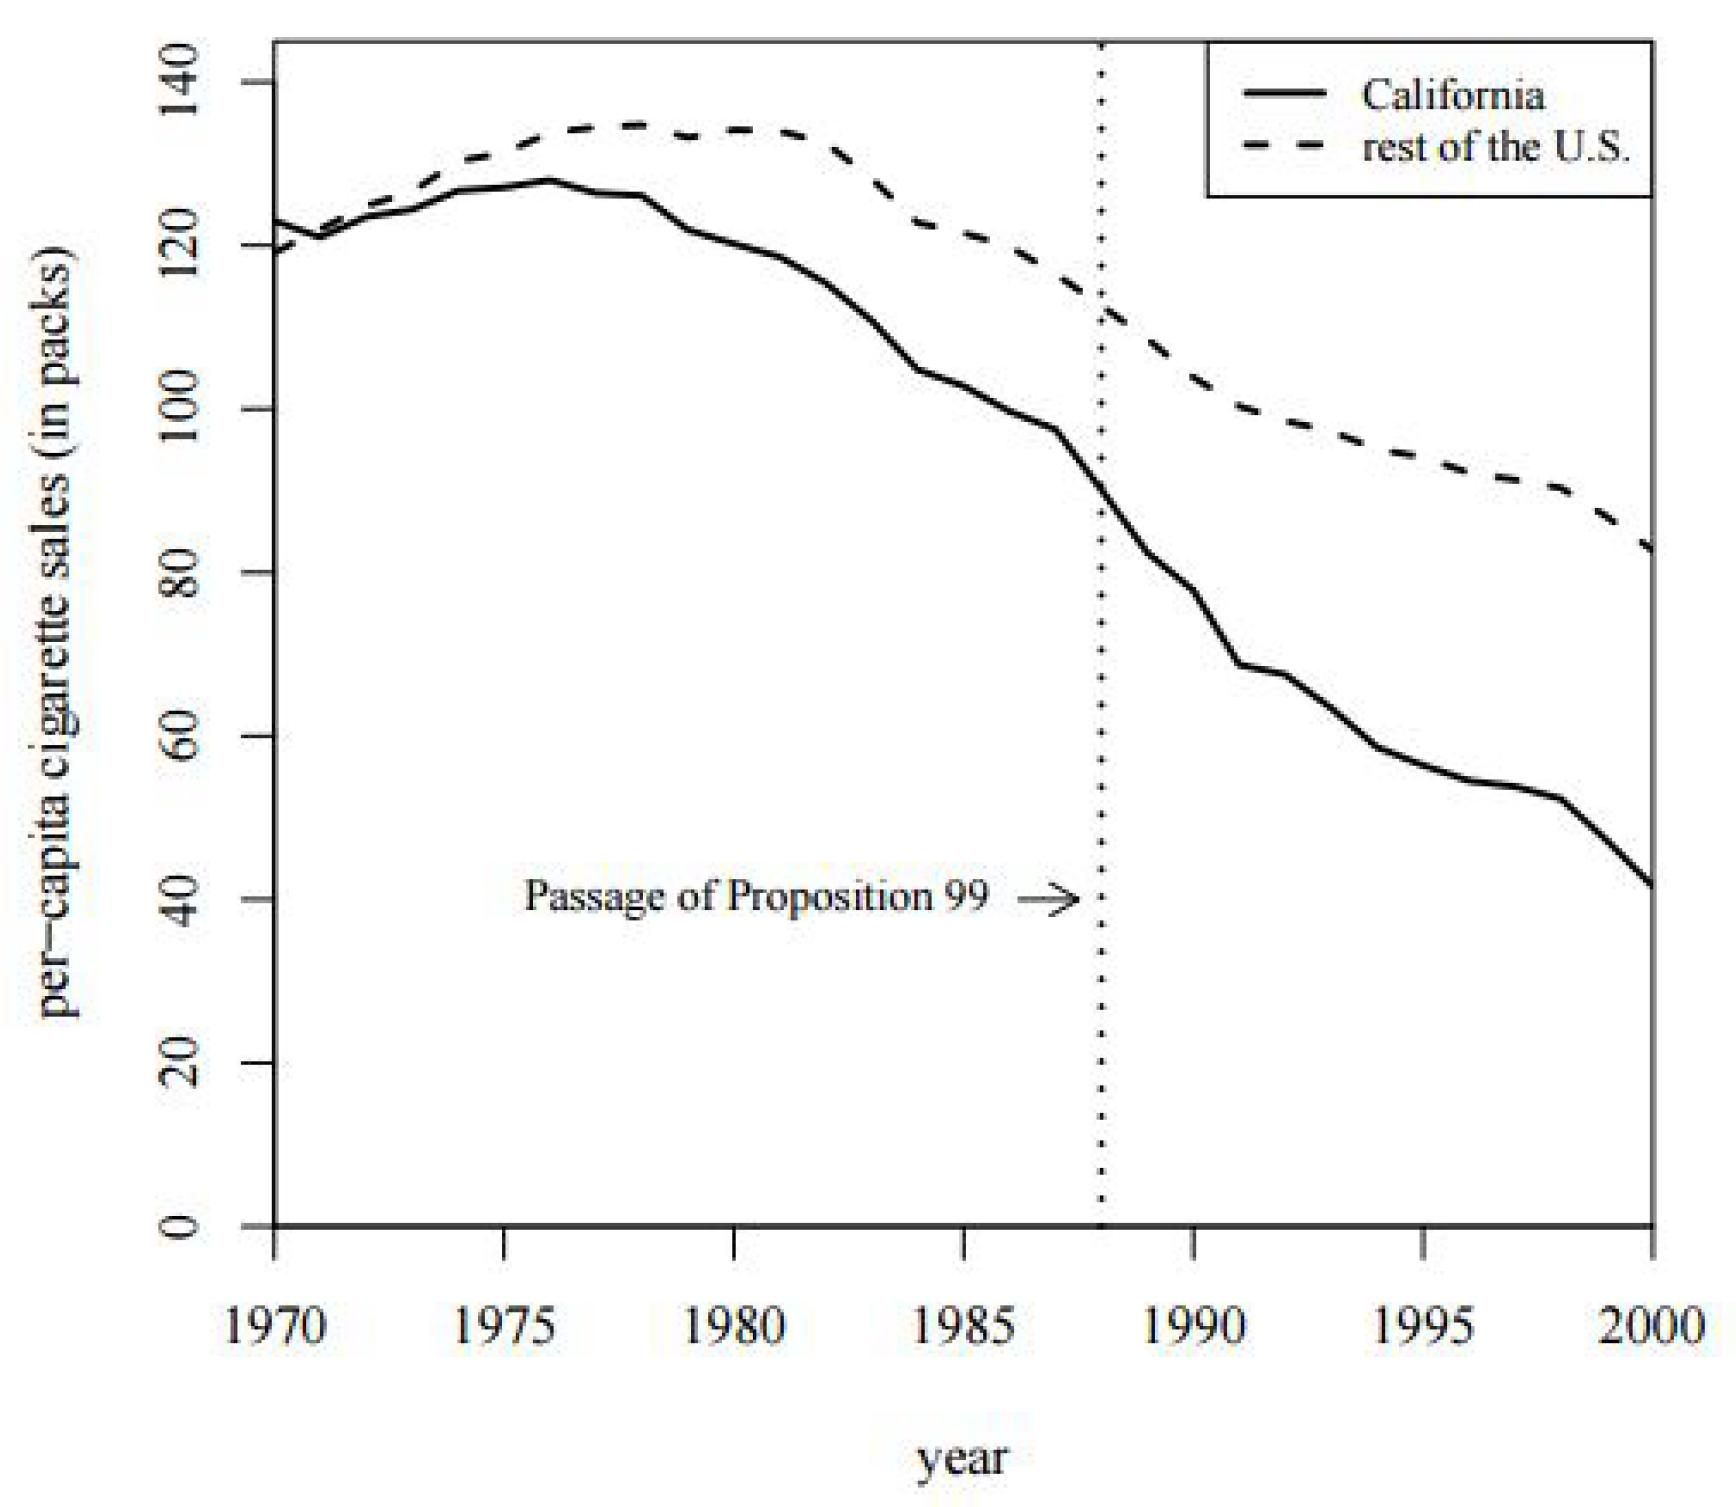
\includegraphics{figure/sc-2.jpg}
\end{figure}
\end{center}
\end{frame}


\begin{frame}{Synthetic Control Method}{Graphical Representation}
\begin{center}
\begin{figure}[p]
\centering
%\scalebox{0.98}{\includegraphics{did_1.jpg}}
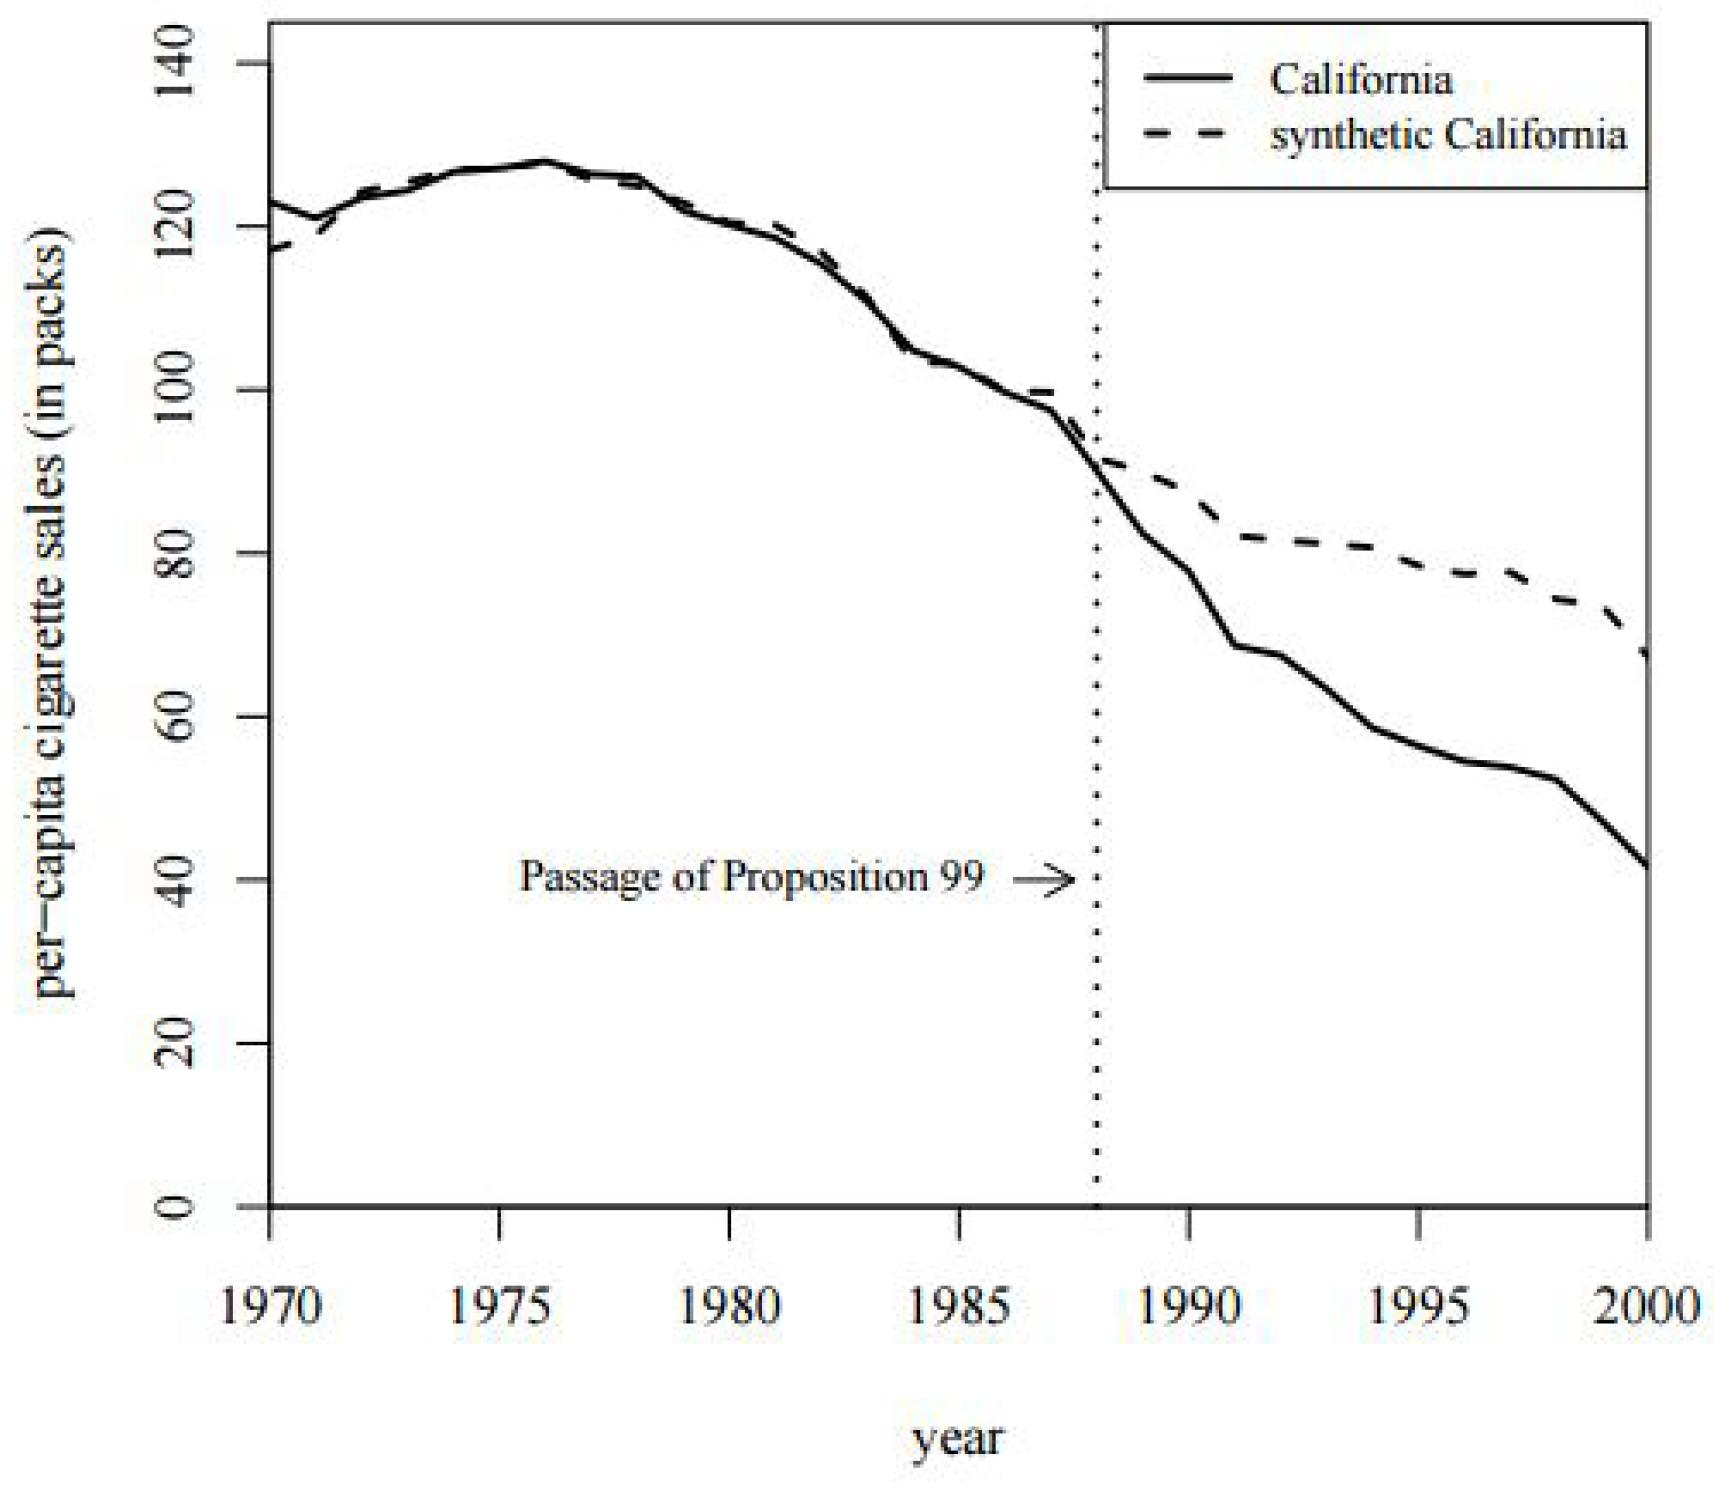
\includegraphics{figure/sc-1.jpg}
\end{figure}
\end{center}
\end{frame}


%\begin{frame}{SC v.s. DID}{Advantages}
%\begin{itemize}
%\item SC builds upon the setting of the standard DID design, but makes the following changes:
%\begin{itemize}
%\vspace{0.2cm}
%%\item[1.] Synthetic Control allows for time-varying individual-specific heterogeneity
%%\vspace{0.2cm}
%
%\item[1] It works in the case where only a single (or small number) of units exposed to the treatment
%\begin{itemize}
%\vspace{0.2cm}
%\item Seek to compensate for the lack of parallel trends 
%by reweighting units to match their pre-exposure trends
%\end{itemize}
%\vspace{0.2cm}
%\item[2] SC takes a serious, data driven approach to forming counterfactuals/selecting the control group
%\vspace{0.2cm}
%\begin{itemize}
%\item  Data-driven procedures reduce discretion in the choice of the control group
%\vspace{0.2cm}
%\end{itemize}
%
%
%\end{itemize}
%\end{itemize}
%\end{frame}
%
%
%
%\begin{frame}{SC v.s. DID}{Disadvantages}
%\begin{itemize}
%\item The benefits of SC method come with three costs:
%\begin{itemize}
%\vspace{0.2cm}
%\item[1.] Large scale (asymptotic) inference cannot be conducted on SC estimators
%\begin{itemize}
%\vspace{0.2cm}
%\item Instead, SC uses \textbf{permutation method} to do statistical inference (compute p-value)
%\vspace{0.2cm}
%\item Recent econometric literature provides new methods for statistical inference
%
%\end{itemize}
%\vspace{0.2cm}
%\item[2.] A key identification assumption is somewhat ambiguous
%\vspace{0.2cm}
%\item[3.] Computational time far exceeds that of DID estimators
%\end{itemize}
%\end{itemize}
%\end{frame}





\begin{frame}{SC v.s. DID}{}
	\begin{itemize}
	
		
		
			\item Treatment Units:
				\vspace{0.2cm}
		\begin{itemize}
			\item DiD: Naturally accommodates multiple treated units
				\vspace{0.2cm}
			\item SCM: Originally designed for a single treated unit 
            				\vspace{0.2cm}
		\end{itemize}
		
		
		\item Control Group Construction:
						\vspace{0.2cm}
		\begin{itemize}
			\item DID: Uses all untreated units with equal weights and require parallel trends assumption
								\vspace{0.2cm}
			\item SCM: Constructs a synthetic control through data-driven weighted average
		\end{itemize}
		\vspace{0.2cm}
		
		
		
		
		
		
	
	\end{itemize}
\end{frame}



\begin{frame}{SC v.s. DID}{}
	\begin{itemize}
		
		
		
		
		
		\item Data Requirements:
										\vspace{0.2cm}
		\begin{itemize}
			\item DID: Works with limited pre-treatment data 
											\vspace{0.2cm}
			\item SCM: Requires extended pre-treatment periods to construct reliable counterfactual
		\end{itemize}
		\vspace{0.2cm}
		
		
		\item Inference Approach:
										\vspace{0.2cm}
		\begin{itemize}
			\item DID: Typically relies on asymptotic statistical inference
												\vspace{0.2cm}
			\item SCM: Uses placebo tests and permutation-based inference
		\end{itemize}
		\vspace{0.2cm}
		
		
		
		
	\end{itemize}
\end{frame}





\title[]  
{Identification}


\author 
{}

%\institute{Institute of Economics, Academia Sinica  \\ Econ, NTU}
%\institute{Institute of Economics, Academia Sinica  \\ IMES/IDAS, NCCU}
\institute{}

%\author 
%{楊子霆 \\ 中研院經濟所}

%\institute 
%{中正大學國際經濟專題研討}




\date
{}


\begin{frame}{}
	\titlepage
\end{frame}




\begin{frame}{Basic Setup: Single Treated Model}{Example}
Alberto Abadie, Alexis Diamond, and Jens Hainmueller (2010), ``\textbf{Synthetic control methods for comparative case studies: Estimating the effect of California's Tobacco Control Program}", Journal of the American Statistical Association	
\begin{itemize}
\vspace{0.2cm}
\item This is one of the first papers using SC method
\vspace{0.2cm}
\begin{itemize}
\item Use this example to go through the key concepts of SC method	
	\vspace{0.2cm}
\item Apply SC method to study the effects of Proposition 99, a large-scale tobacco control program that California implemented in 1988	
\vspace{0.2cm}	
\item A single treated unit with multiple non-treated units		
\end{itemize}	

\end{itemize}
\end{frame}



\begin{frame}{Basic Setup: Single Treated Model}{Example}
\begin{itemize}
\item In 1988, California passed comprehensive tobacco control legislation:
\begin{itemize}
\vspace{0.2cm}
\item Increased cigarette taxes by \$0.25 per pack
\vspace{0.2cm}
\item Funded anti-smoking media campaigns
\vspace{0.2cm}
\item Spurred clean-air ordinances
\end{itemize}
\vspace{0.2cm}
\item They want to estimate the causal effect of the policy on cigarette consumption in California
%\vspace{0.2cm}
%\item Other states that subsequently passed control programs excluded from control group
\end{itemize}
\end{frame}







\begin{frame}{Basic Setup: Single Treated Model}
\begin{itemize}
\item Suppose we observe $J+1$ units over $t=1,...,T$ periods
%with unit $1$ being treated and units $\{2,...,J+1\}$ being unaffected
\vspace{0.2cm}
\item A ``treatment" occurs at period $T_0+1$
\vspace{0.2cm}
\begin{itemize}	
\item Unit $1$ being treated
\vspace{0.2cm}
\item Units $\{2,...,J+1\}$ being unaffected 
\vspace{0.2cm}
\item Pre-treatment period: $1,\ldots,T_0$	
\vspace{0.2cm}	
\item Post-treatment period: $T_0+1,\ldots,T$	
\vspace{0.2cm} 
\end{itemize}
%affects unit $1$ only, and leaves the other $J$ states unaffected 

\item We aim to identify the causal effect of the treatment on unit $1$

\vspace{0.2cm} 
\begin{itemize}
\item Individual treatment effect for unit $1$
\end{itemize}
\end{itemize}

\end{frame}


\begin{frame}{Potential Outcomes Framework}{}
	\begin{itemize}
		
		\item \textcolor{blue}{Treatment}
		\begin{itemize}
			\vspace{0.2cm}
			\item $D_{it}=1$: the units that are treated from periods $T_0+1$ until $T$
			\vspace{0.2cm}
			\item $D_{it}=0$: the units that are always untreated
		\end{itemize}
		
	\end{itemize}
\end{frame}




\begin{frame}{Potential Outcomes Framework}{}
\begin{itemize}
\item \textcolor{blue}{Potential Outcomes}
\vspace{0.2cm}
\begin{itemize}
\item $\mathrm{Y}^{1}_{it}$: the potential outcome we \textit{would} observe for unit $i$ at time $t$ if unit $i$ receives the treatment 
\vspace{0.2cm}
\begin{itemize}
\item Note that the treated unit would receive treatment from periods $T_0+1$ until $T$
\end{itemize}
\vspace{0.2cm}
\item $\mathrm{Y}^{0}_{it}$: the potential outcome we \textit{would} observe for unit $i$ at time $t$ if unit $i$ does not receive the treatment
\end{itemize}
\vspace{0.2cm}
\item Note that \textbf{unit in synthetic control method is usually aggregate level}: country, state, county, or region 



\end{itemize}
\end{frame}









\begin{frame}{Potential Outcomes Framework}{}
\begin{itemize}

\item \textcolor{blue}{Observed Outcomes}
\vspace{0.2cm}
\begin{itemize}
\item $Y_{it}$ is the observed outcome for unit $i$ at time $t$
\vspace{0.2cm}	
\begin{itemize}
\item Observed outcomes before period $T_0+1$:

\begin{equation*}
Y_{it}=\mathrm{Y}^{0}_{it}
\end{equation*}
\item Observed outcomes after period $T_0+1$: 
\begin{equation*}
Y_{it}=\mathrm{Y}^{0}_{it}(1-D_{it})+\mathrm{Y}^{1}_{it}D_{it}
\end{equation*}
%\item Treatment effect for unit $i$ at time $t=1$ is
%	\begin{equation*}
%	\mathrm{Y}^{1}_{i1}-\mathrm{Y}^{0}_{i1}
%	\end{equation*}
\end{itemize}
\end{itemize}


\end{itemize}
\end{frame}





\begin{frame}{Potential Outcomes Framework}{}
\begin{itemize}
\item Since only unit $1$ is treated, we aim to estimate the causal effect of treatment over time ($T_{0}+1,.....,T$) for the treated unit $1$
\begin{equation*}
\alpha_{1t}=(\alpha_{1T_{0}+1},...,\alpha_{1T})
\end{equation*}
where for $t>T_0$:
\begin{equation*}
\alpha_{1t}=\underbrace{Y^1_{1t}}_{\text{observed}}-\underbrace{Y^0_{1t}}_{\text{counterfactual}}
\end{equation*}
\vspace{0.2cm}
\item We need to construct the \textbf{unobserved counterfactual} for unit $1$
\end{itemize}
\end{frame}









\title[]  
{Estimation}


\author 
{}

%\institute{Institute of Economics, Academia Sinica  \\ Econ, NTU}
%\institute{Institute of Economics, Academia Sinica  \\ IMES/IDAS, NCCU}
\institute{}

%\author 
%{楊子霆 \\ 中研院經濟所}

%\institute 
%{中正大學國際經濟專題研討}




\date
{}


\begin{frame}{}
\titlepage
\end{frame}




\begin{frame}{SC Estimation}




\begin{equation*}
\alpha_{1t}=\underbrace{Y^1_{1t}}_{\text{observed}}-\underbrace{Y^0_{1t}}_{\text{counterfactual}}
\end{equation*}	
\begin{itemize}
\item SC method suggests treatment effect can be estimated by the simple difference:

\begin{equation*}
\hat{\alpha}_{1t}=Y_{1t}-\sum^{J+1}_{i=2}w^*_{i}Y_{it}
\end{equation*}
	

\end{itemize}
\end{frame}






\begin{frame}{SC Estimation}
\begin{itemize}
	\item Choose weights $W=(w^{*}_{2},...,w^{*}_{J+1})$$\in$ [0,1] to minimize difference in pre-treatment characteristics $X$ between treated and weighted average of non-treated units
	\vspace{0.2cm}
	\begin{equation*}
		\begin{aligned}
			W^* = \argmin\limits_{W} & \sum_{k=1}^{K} v_k\left(X_{1k} - \sum_{i=2}^{J+1} w_i X_{ik}\right)^2 \\
			\text{subject to } & \sum_{i=2}^{J+1} w_i = 1, \; w_i \geq 0 \;\forall\, i \in \{2,\ldots,J+1\}
		\end{aligned}
\end{equation*}

\begin{itemize}
	\item $X_{1k}$ is the $k$-th predictor variable for the treated unit
				\vspace{0.2cm}
		\item $X_{ik}$ is the $k$-th predictor variable for non-treated unit $i$
					\vspace{0.2cm}
			\item $v_k$ represents relative importance of each predictor variable (chosen by cross-validation)
\end{itemize}
\end{itemize}
\end{frame}


\begin{frame}{SC Estimation}{Choosing $v_k$: Intuition}
\begin{itemize}
	\item $v_k$ controls how much weight predictor $k$ receives when measuring ``closeness'' between the treated unit and the synthetic unit
	\vspace{0.2cm}
	\begin{itemize}
		\item A \textbf{larger} $v_k$ $\Rightarrow$ predictor $k$ must be matched more precisely
		\vspace{0.2cm}
		\item A \textbf{smaller} $v_k$ $\Rightarrow$ predictor $k$ matters less in constructing the synthetic unit
	\end{itemize}
	\vspace{0.2cm}
	\item \textbf{Key question:} Which predictors are most informative for reproducing the pre-treatment outcome trajectory?
	\vspace{0.2cm}
	\begin{itemize}
		\item We want $v_k$ to be \textbf{large} for predictors that help fit pre-treatment $Y_{1t}$ well
	\end{itemize}
\end{itemize}
\end{frame}


\begin{frame}{SC Estimation}{Choosing $v_k$: Cross-Validation}
\begin{itemize}
	\item Split the pre-treatment period into two sub-periods:
	\vspace{0.2cm}
	\begin{itemize}
		\item \textbf{Training period:} $1,\ldots,T_1$ \quad (``in-sample'')
		\vspace{0.2cm}
		\item \textbf{Validation period:} $T_1{+}1,\ldots,T_0$ \quad (``out-of-sample'')
	\end{itemize}
	\vspace{0.2cm}
	\item \textbf{Nested (bilevel) optimization:}
	\vspace{0.1cm}
	\begin{itemize}
		\item \textbf{Inner problem} (given $V$): find $W^{*}(V)$ that minimizes predictor mismatch \textit{in the training period}
		\vspace{0.1cm}
		\item \textbf{Outer problem}: choose $V^{*}$ to minimize out-of-sample prediction error \textit{in the validation period}:
		\begin{equation*}
			V^{*} = \argmin_{V} \sum_{t=T_1+1}^{T_0}
			\left(Y_{1t} - \sum_{i=2}^{J+1} w^{*}_{i}(V)\,Y_{it}\right)^{2}
		\end{equation*}
	\end{itemize}
	\item \textbf{Intuition:} Pick $v_k$'s so that the synthetic unit fitting predictors well \textit{also} predicts the outcome well in the portion of the pre-treatment period it has not yet ``seen''
\end{itemize}
\end{frame}





\begin{frame}{SC Estimation}
	\begin{itemize}
		
	\item Predictor variables $X$ typically include:
				\vspace{0.2cm}
			\begin{itemize}
					\item Pre-treatment outcomes $Y_{1},...,Y_{T_0}$ (most predictive)
								\vspace{0.2cm}
					\item Other observed covariates $Z$ 
				\end{itemize}
			\vspace{0.2cm}
			\item Different predictor variables $X$ and choice of weights $v_k$ result in distinct synthetic units
	\end{itemize}
\end{frame}





%\begin{frame}{Synthetic Control Method (SCM) Estimation - I}
%	\begin{itemize}
%		\item Create a "synthetic control unit" by weighted averaging of non-treated units to match pre-treatment characteristics of the treated unit
%		\vspace{0.2cm}
%		\item Choose weights $W=(w_{2},...,w_{J+1})$ $\in$ [0,1] to minimize difference in pre-treatment characteristics $X$ between treated and weighted average of non-treated units:
%		\vspace{0.2cm}
%		\begin{equation*}
%			\begin{aligned}
%				W^* = \argmin\limits_{W} & \sum_{k=1}^{K} v_k\left(X_{1k} - \sum_{j=2}^{J+1} w_j X_{jk}\right)^2 \\
%				\text{subject to } & \sum_{j=2}^{J+1} w_j = 1, \; w_j \geq 0 \; \forall j \in \{2,...,J+1\}
%			\end{aligned}
%		
%\end{equation*}
%		\item Where:
%		\begin{itemize}
%			\item $X_{1k}$ is the $k$-th predictor variable for the treated unit
%			\item $X_{jk}$ is the $k$-th predictor variable for non-treated unit $j$
%			\item $v_k$ represents relative importance of each predictor variable (typically chosen by cross-validation)
%		\end{itemize}
%	\end{itemize}
%\end{frame}
%
%\begin{frame}{Synthetic Control Method (SCM) Estimation - II}
%	\begin{itemize}
%		\item Predictor variables $X$ typically include:
%		\begin{itemize}
%			\item Pre-treatment outcomes $Y_{1},...,Y_{T_0}$ (most predictive)
%			\item Other observed covariates $Z$ (demographics, economic indicators, etc.)
%		\end{itemize}
%		\vspace{0.3cm}
%		\item Different predictor variables $X$ and choice of weights $v_k$ result in distinct synthetic units
%		\vspace{0.3cm}
%		\item Treatment effect estimation:
%		\begin{equation*}
%			\hat{\tau}_{1t} = Y_{1t} - \sum_{j=2}^{J+1} w^*_j Y_{jt}, \quad \forall t > T_0
%		
%\end{equation*}
%		\vspace{0.2cm}
%		\item Method advantages:
%		\begin{itemize}
%			\item No need for random assignment of treatment
%			\item Allows for time-varying treatment effects
%			\item Transparent weight selection process
%			\item Avoids extrapolation issues
%		\end{itemize}
%	\end{itemize}
%\end{frame}




\begin{frame}{Assumptions of SC}
	\begin{itemize}
		\item Assume potential outcome if unit $1$ would not receive treatment $Y^0_{1t}$ can be expressed as follows:
		\begin{equation*}
			Y^0_{1t}=\delta_t+\theta_tZ_1+\lambda_t\mu_1+\varepsilon_{1t}
\end{equation*}
		\begin{itemize}
			\item $\delta_t$ are common time effects (e.g. year fixed effects)
			\vspace{0.2cm}
			\item $Z_1$ are the observed, pre-treatment covariates
			\vspace{0.2cm}
			\item $\mu_1$ are \textbf{permanent} unobserved variables
			\vspace{0.2cm}
			\item $\varepsilon_{1t}$ are unobserved transitory shocks at the unit level with zero mean
			\vspace{0.2cm}
		\end{itemize}
		\item This assumption allows time-varying responses of multiple unobserved factors ($\lambda_t\mu_1$) 
		
		%heterogenous responses to multiple unobserved factors ($\lambda_t\mu_i$) 
		%and embeds time-trend models
		\vspace{0.2cm}
		\item However, it implicitly assumes \textbf{the unobservable factor loadings $\mu_i$ are fixed over time} 
		\vspace{0.2cm}
		\begin{itemize}
			\item No structural breaks
		\end{itemize}
		
		
	\end{itemize}
\end{frame}



%\begin{frame}{Why SCM Relaxes the Parallel Trends Assumption}
%	\begin{itemize}
%		\item Recall the factor model: $Y^0_{1t}=\delta_t+\theta_tZ_1+\lambda_t\mu_1+\varepsilon_{1t}$
%		\vspace{0.2cm}
%		
%		\item SCM creates a synthetic control by selecting weights $W^*$ such that:
%		\begin{equation*}
%			\sum_{j=2}^{J+1} w^*_j Y_{jt} \approx Y_{1t} \text{ for } t < T_0
%		
%\end{equation*}
%		
%		\item This implicitly ensures:
%		\begin{equation*}
%			\sum_{j=2}^{J+1} w^*_j \mu_j \approx \mu_1 \text{ and } \sum_{j=2}^{J+1} w^*_j Z_j \approx Z_1
%		
%\end{equation*}
%		
%		\vspace{0.2cm}
%		
%		\item Three key advantages over DiD:
%		\begin{itemize}
%			\item \textbf{Non-parallel pre-treatment trends}: By matching the entire pre-treatment trajectory, SCM captures unit-specific trends rather than assuming parallel paths
%			\vspace{0.2cm}
%			
%			\item \textbf{Time-varying effects of unobserved variables}: The term $\lambda_t\mu_1$ allows unobserved factors to have different effects at different time points
%			\vspace{0.2cm}
%			
%			\item \textbf{Heterogeneous responses to common shocks}: Units with different characteristics ($\mu_j$) can respond differently to common time effects, and SCM accounts for this by matching these characteristics
%		\end{itemize}
%		
%		\vspace{0.2cm}
%		
%		\item Example: During economic recessions ($\delta_t$), regions with different industrial compositions ($\mu_j$) may experience different impacts—SCM can capture this heterogeneity
%	\end{itemize}
%\end{frame}




\begin{frame}{SC Estimation}
\begin{itemize}

\item Ideally, one would want to select $W^{*}$ such that

\begin{equation*}
\sum^{J+1}_{j=2}w^*_{j}Z_{j} = Z_{1}  
\end{equation*}

\begin{equation*}
\sum^{J+1}_{j=2}w^*_{j}\mu_{j} = \mu_{1}  
\end{equation*}

\item Thus, causal effect of treatment $\hat{\alpha}_{1t}$ is unbiased 	

\end{itemize}
\end{frame}







\begin{frame}{SC Estimation}
\begin{itemize}
	
	\item Problem: \textbf{$\mu_{i}$ is unobserved}
\end{itemize}
\end{frame}





\begin{frame}{SC Estimation}
\begin{itemize}

\item Solution: Choose $W=(w^{*}_{2},...,w^{*}_{J+1})$ satisfying

\begin{equation*}
\begin{aligned}
&\sum^{J+1}_{i=2}w^*_{i}Z_{i} = Z_{1}, \\ 
&\sum^{J+1}_{i=2}w^*_{i}Y_{i1} = Y_{11},  \\
&\sum^{J+1}_{i=2}w^*_{i}Y_{i2} = Y_{12},...,  \\
&\sum^{J+1}_{i=2}w^*_{i}Y_{iT_{0}} = Y_{1T_{0}}    
\end{aligned}
\end{equation*}

\end{itemize}
\end{frame}






\begin{frame}{SC Estimation}
\begin{itemize}
\item \textbf{SC Theorem}: Suppose there exists $W^*$ such that the SC matches the treated unit in the pre-treatment period ($\forall t\in\{1,...,T_0\}$): 
\begin{align*}
\sum^{J+1}_{i=2}w^*_{i}Y_{it}&=Y_{1t} \\
\sum^{J+1}_{i=2}w^*_{i}Z_i&=Z_1,
\end{align*}
and $\sum^{T_0}_{t=1}\lambda'_t\lambda_t$ is non-singular. Then for all $t>T_0$ we have
\begin{equation*}
\mathbb{E}\left[Y^0_{1t}-\sum^{J+1}_{i=2}w^*_{i}Y_{it}\right]\rightarrow 0
\end{equation*}
as $T_0\rightarrow\infty$ 

%or if $T_0$ is large relative to $\varepsilon_{i,t}$
\end{itemize}
\end{frame}


%
%\begin{frame}{SC: Model Setup}
%	\begin{itemize}
%		\item \textbf{Data Generating Process}:
%		\begin{equation*}
%			Y_{it} = \delta_t + \theta_t Z_i + \lambda_t \mu_i + \epsilon_{it}
%		
%\end{equation*}
%		where
%		\begin{itemize}
%			\item $\delta_t$: time fixed effects (e.g., general economic conditions)
%			\item $\theta_t Z_i$: observed characteristics with time-varying coefficients
%			\item $\lambda_t \mu_i$: unobserved common factors ($\lambda_t$) with unit-specific loadings ($\mu_i$)
%			\item $\epsilon_{it}$: transitory shocks
%		\end{itemize}
%	\end{itemize}
%\end{frame}
%\begin{frame}{SC: Identification}
%	\begin{itemize}
%		\item If there exists weights $W^$ such that:
%		\begin{align}
%			\sum_{j=2}^{J+1} w_j^* Z_j &= Z_1 \text{ (matching on observables)}\
%			\sum_{j=2}^{J+1} w_j^* \mu_j &= \mu_1 \text{ (matching on factor loadings)}
%		\end{align}
%		\item Then the synthetic control will approximate the counterfactual:
%		\begin{equation*}
%			Y_{1t}^0 \approx \sum_{j=2}^{J+1} w_j^* Y_{jt}
%		
%\end{equation*}
%		\item The condition $\sum_{t=1}^{T_0} \lambda_t'\lambda_t$ non-singular ensures:
%		\begin{itemize}
%			\item Common factors are linearly independent
%			\item Sufficient variation to identify factor loadings
%			\item Pre-treatment fit implies matching on factor loadings
%		\end{itemize}
%	\end{itemize}
%\end{frame}
%
%
%\begin{frame}{SC: Implementation}
%	\begin{itemize}
%		\item In practice, we:
%		\begin{equation*}
%			\begin{aligned}
%				W^* = \argmin\limits_{W} & \sum_{k=1}^{K} v_k\left(X_{1k} - \sum_{j=2}^{J+1} w_j X_{jk}\right)^2 \
%				\text{subject to } & \sum_{j=2}^{J+1} w_j = 1, \quad w_j \geq 0
%			\end{aligned}
%		
%\end{equation*}
%		\item Where $X$ includes both $Z$ and pre-treatment $Y$
%		\item Good pre-treatment fit suggests we've matched on both:
%		\begin{itemize}
%			\item Observable characteristics ($Z$)
%			\item Unobservable factor loadings ($\mu$)
%		\end{itemize}
%	\end{itemize}
%\end{frame}





\begin{frame}{SC Estimation}{Graphical Representation}
\begin{center}
	\begin{figure}[p]
		\centering
		%\scalebox{0.98}{\includegraphics{did_1.jpg}}
		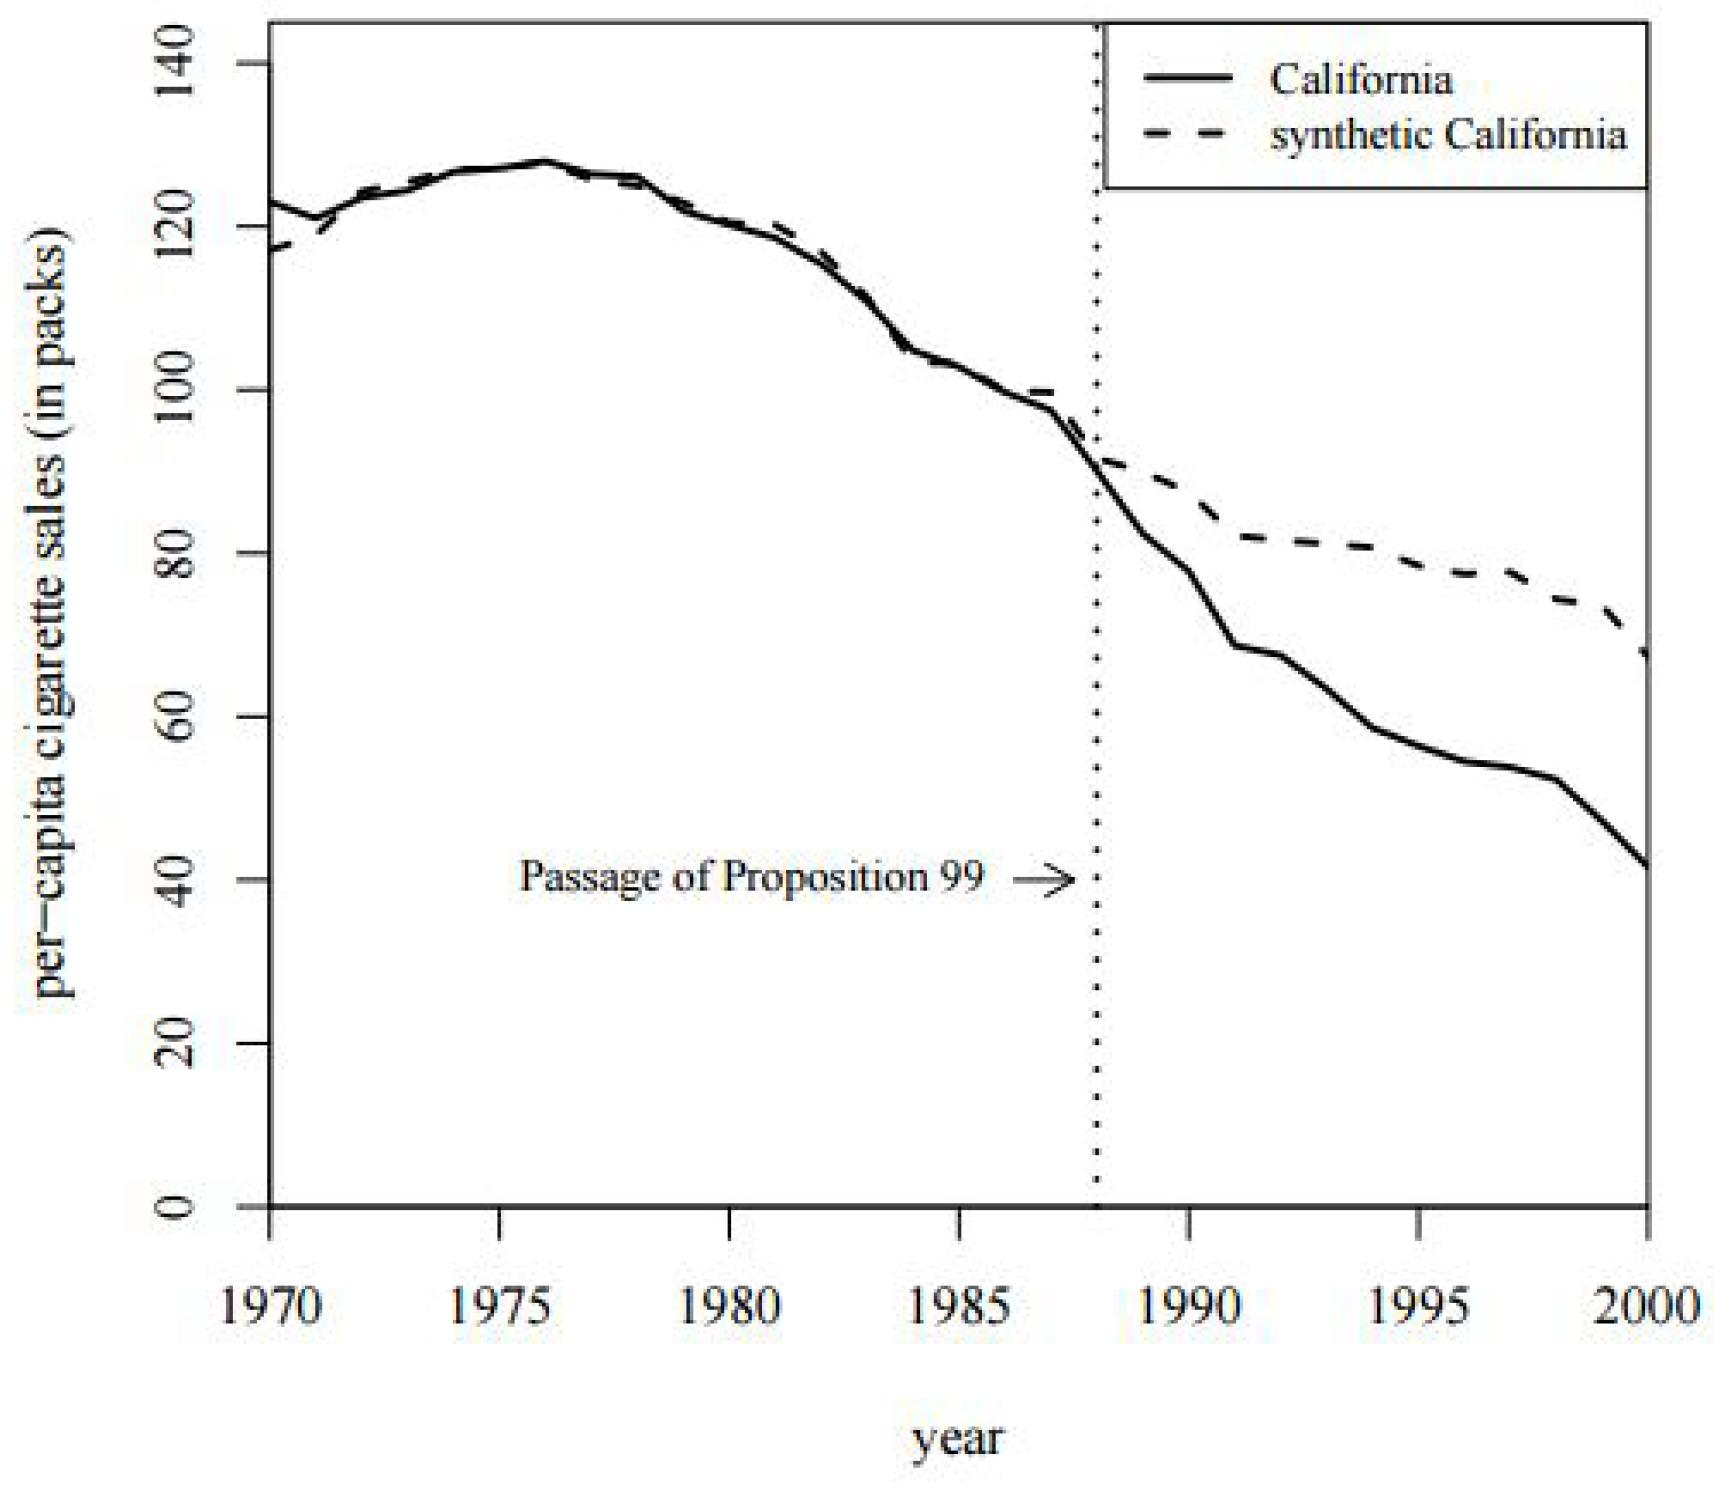
\includegraphics{figure/sc-1.jpg}
	\end{figure}
\end{center}
\end{frame}



\begin{frame}{SC Estimation}{Intuition}
\begin{itemize}
%\item If the conditions are met, the the ``synthetic control" associated with $W^*$ replicates the missing counterfactual
%\vspace{0.2cm}
\item An approximately unbiased estimator of causal effect of treatment $\alpha_{1t}$ is then given by:
\begin{equation*}
\hat{\alpha}_{1t}=Y_{1t}-\sum^{J+1}_{i=2}w^*_iY_{it}
\end{equation*}

\begin{itemize}
\item The difference between the observed outcome and the outcome of synthetic unit.

\end{itemize}

\vspace{0.2cm}
\item Beauty of SC is that even though the \textbf{$\mu_1$ are unobservable}, fitting $\{Y_{1t},Z_{1}\}$ is sufficient to match the process
\vspace{0.2cm}
\item \textbf{Intuition:} a synthetic cohort can fit ($Z_{1},Y_{11},...Y_{1T_{0}} $) for a large $T_{0}$ only if it fits ($Z_{1},\mu_{1} $)
\end{itemize}
\end{frame}


%\begin{frame}{Why SCM Relaxes the Parallel Trends Assumption}
%	\begin{itemize}
%	
%			\item DID design requires that the difference between treated and untreated units remains constant over time in the absence of treatment (Parallel Trends Assumption)
%			
%			
%			
%			\item By matching the entire pre-treatment trajectory, SC captures unit-specific trends rather than assuming parallel trend
%			
%
%			
%			
%		
%			
%		
%	\end{itemize}
%\end{frame}



%\begin{frame}{Why SCM Relaxes the Parallel Trends Assumption}
%	\begin{itemize}
%		\item \textbf{DiD Assumption}: In the absence of treatment, the difference between treated and control units would remain constant over time (Parallel Trends)
%		\vspace{0.3cm}
%		
%		\item \textbf{DiD Factor Model}: $Y^0_{it} = \alpha_i + \delta_t + \varepsilon_{it}$
%		\begin{itemize}
%			\item Time-invariant unit effects ($\alpha_i$) + common time effects ($\delta_t$)
%		\end{itemize}
%		\vspace{0.3cm}
%		
%		\item \textbf{SCM Approach}: Instead of assuming parallel trends, SCM creates a counterfactual by:
%		\begin{itemize}
%			\item Matching the entire pre-treatment trajectory of the treated unit
%			\item Allowing for time-varying effects of unobserved factors ($\lambda_t\mu_i$)
%			\item Directly constructing the control unit as a weighted average of donor units
%		\end{itemize}
%		\vspace{0.3cm}
%		
%		\item \textbf{Implication}: SCM can accommodate non-parallel trends and heterogeneous responses to common shocks across units
%	\end{itemize}
%\end{frame}



\begin{frame}{Example: Abadie et al. (2010)}{Results: Unit Weights for SC}
\begin{center}
	\begin{figure}[p]
		\centering
		\scalebox{0.65}{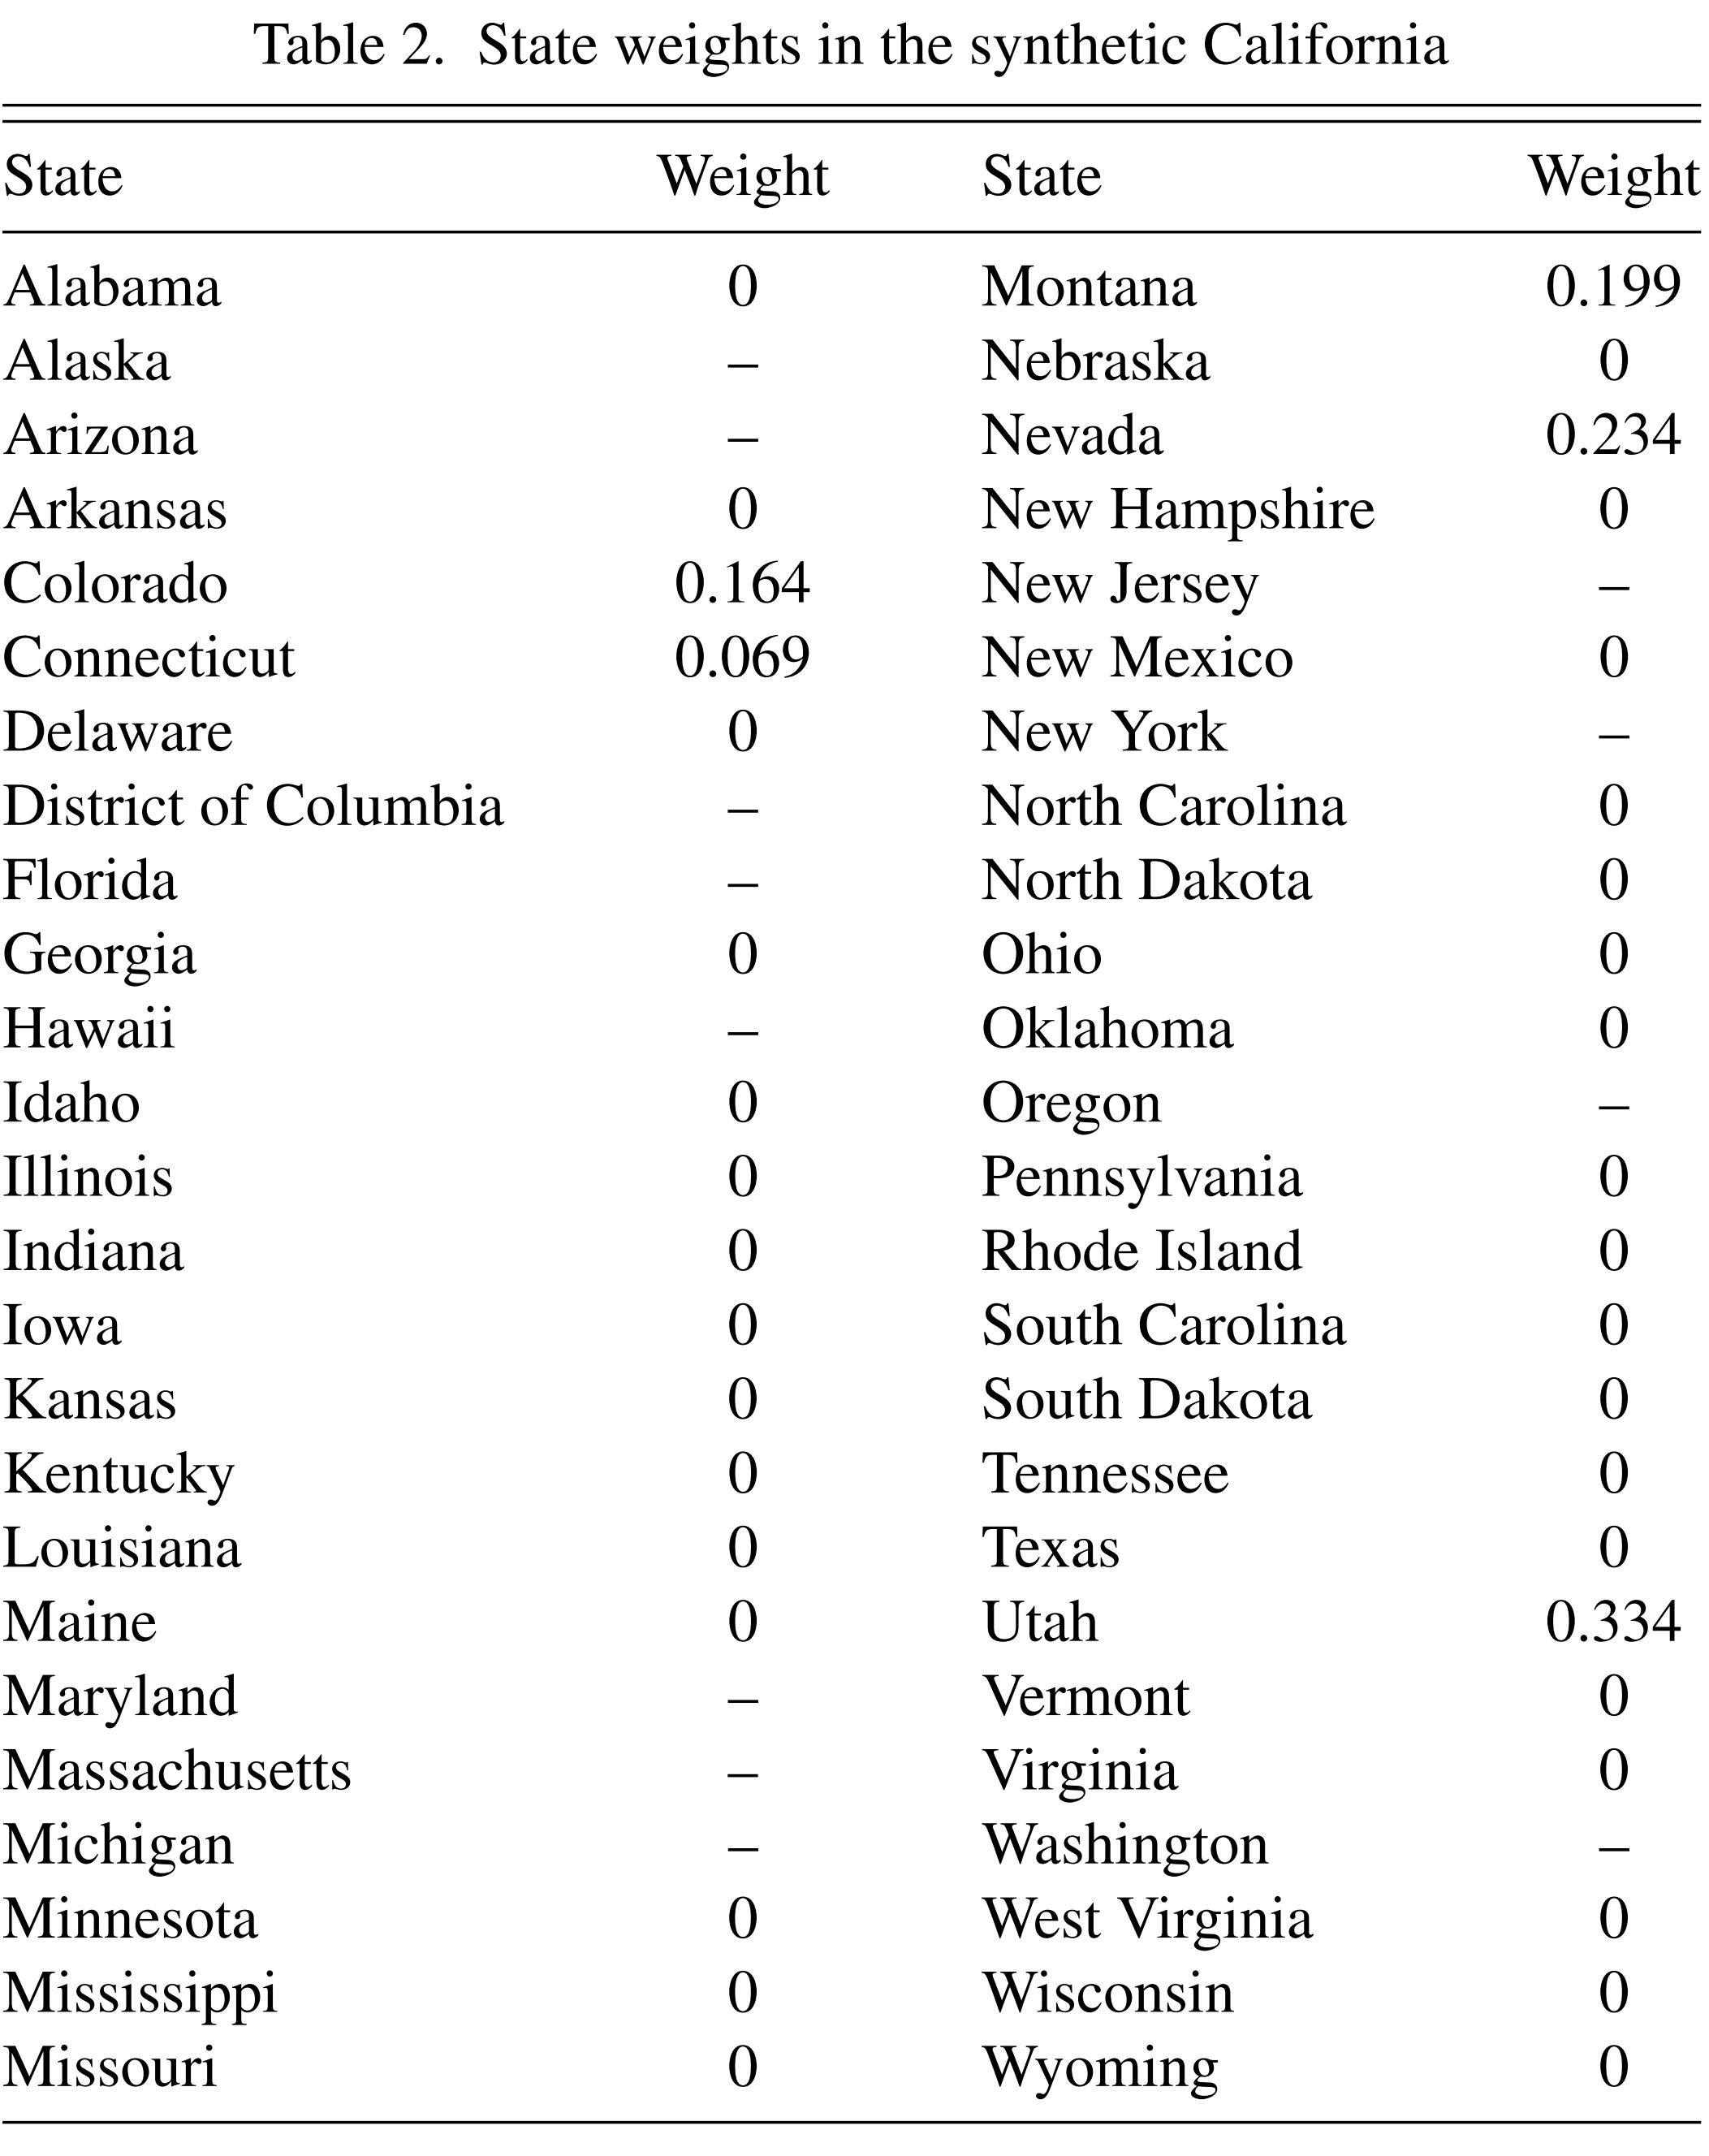
\includegraphics{figure/sc_t2.jpg}}
		%\includegraphics{sc-5.jpg}
	\end{figure}
\end{center}
\end{frame}


\begin{frame}{Example: Abadie et al. (2010)}{Comparison of Synthetic Fit and Simple Average}
\begin{table}[p]
\centering
%\extrarowheight = 3pt 
\scalebox{0.95}{
\begin{tabular}{lccc}
\hline
& \multicolumn{2}{c}{California}    & Average of  \\
Variables & Real        & Synthetic           & 38 control states \\
\hline
Ln (GDP per capita)         & 10.08 & 9.86  & 9.86   \\
Percent aged 15-24          & 17.40 & 17.40 & 17.29  \\
Retail price                & 89.42 & 89.41 & 87.27  \\
Beer consumption per capita & 24.28 & 24.20 & 23.75  \\
Cigarette sales per capita 1988 & 90.10  & 91.62  & 114.20  \\
Cigarette sales per capita 1980 & 120.20 & 120.43 & 136.58  \\
Cigarette sales per capita 1975 & 127.10 & 126.99 & 132.81  \\
\hline
\end{tabular}}
\end{table}
\end{frame}





\title[]  
{Statistical Inference}


\author 
{}

%\institute{Institute of Economics, Academia Sinica  \\ Econ, NTU}
%\institute{Institute of Economics, Academia Sinica  \\ IMES/IDAS, NCCU}
\institute{}

%\author 
%{楊子霆 \\ 中研院經濟所}

%\institute 
%{中正大學國際經濟專題研討}




\date
{}


\begin{frame}{}
	\titlepage
\end{frame}




\begin{frame}{Statistical Inference of SC}
\begin{itemize}
\item Large-sample asymptotic inference is not possible with SC
\vspace{0.2cm}
\item Abadie et al. (2010) suggest the use of \textbf{permutation methods} for inference 
\vspace{0.2cm}
	\begin{itemize}
	%\item Similar to Fisher's exact test
	\item Does not rely on large-sample asymptotics
	%	\item Provides exact inference under exchangeability
\end{itemize}
\vspace{0.2cm}
\item \textbf{Main Idea:} 
\vspace{0.2cm}
\begin{itemize}
\item How often would we obtain results of this magnitude if we had chosen a state at random for the study instead of California ?
\vspace{0.2cm}

\item Run placebo studies by applying the SC method to states that did NOT receive treatment
\vspace{0.2cm}
\begin{itemize}
\item  If the placebo studies create gaps of magnitude similar to the one estimated for California 
\vspace{0.2cm}
\item Then our interpretation is that
our analysis does NOT provide significant evidence of causal effect
\end{itemize}
\end{itemize}
\end{itemize}
\end{frame}










\begin{frame}{Permutation Test: Basic Steps}
	\begin{itemize}
		\item \textbf{Step 1:} Estimate treatment effect for treated unit (e.g., California)
		\begin{equation*}
			\hat{\alpha}_{1t} = Y_{1t} - \sum_{j=2}^{J+1} w_j^* Y_{jt}, \quad t > T_0
\end{equation*}
		\vspace{0.2cm}
		\item \textbf{Step 2:} Conduct placebo studies
				\vspace{0.2cm}
		\begin{itemize}
			\item Apply SC to each control unit in donor pool as if it were treated
					\vspace{0.2cm}
			\item Calculate placebo effects $\{\hat{\alpha}_{2t},...,\hat{\alpha}_{J+1,t}\}$
		%			\vspace{0.2cm}
		%	\item Compare magnitude of effects across units
		\end{itemize}
		\vspace{0.2cm}
		\item \textbf{Key Question:} How unusual is the estimated effect for California compared to effects we estimate for units that did NOT receive treatment?
	\end{itemize}
\end{frame}

\begin{frame}{Permutation Test: Statistical Inference}
	\begin{itemize}
		\item \textbf{Step 3:} Calculate empirical p-value
		\begin{itemize}
			\item Plot all estimated effect (treated and placebos) for visual inspection
			\vspace{0.2cm}
			\item Calculate empirical p-value at each post-treatment time $t$:
			\begin{equation*}
				p_{1t}=\dfrac{\sum^{J+1}_{i=2}\mathbf{1}\{\hat{\alpha}_{it}\geq\hat{\alpha}_{1t}\}}{J}
\end{equation*}
			where $\mathbf{1}\{\cdot\}$ is the indicator function
		\end{itemize}
		\vspace{0.2cm}
		\item \textbf{Interpretation:} 
		\begin{itemize}
			\item Small $p_{1t}$: treatment effect is unusually large compared to placebo effects
					\vspace{0.2cm}
			\item Large $p_{1t}$: cannot distinguish treatment effect from random chance
		\end{itemize}
	\end{itemize}
\end{frame}


\begin{frame}{SC Analysis for Treated State}{California}
	\begin{center}
		\begin{figure}[p]
			\centering
			%\scalebox{0.98}{\includegraphics{did_1.jpg}}
			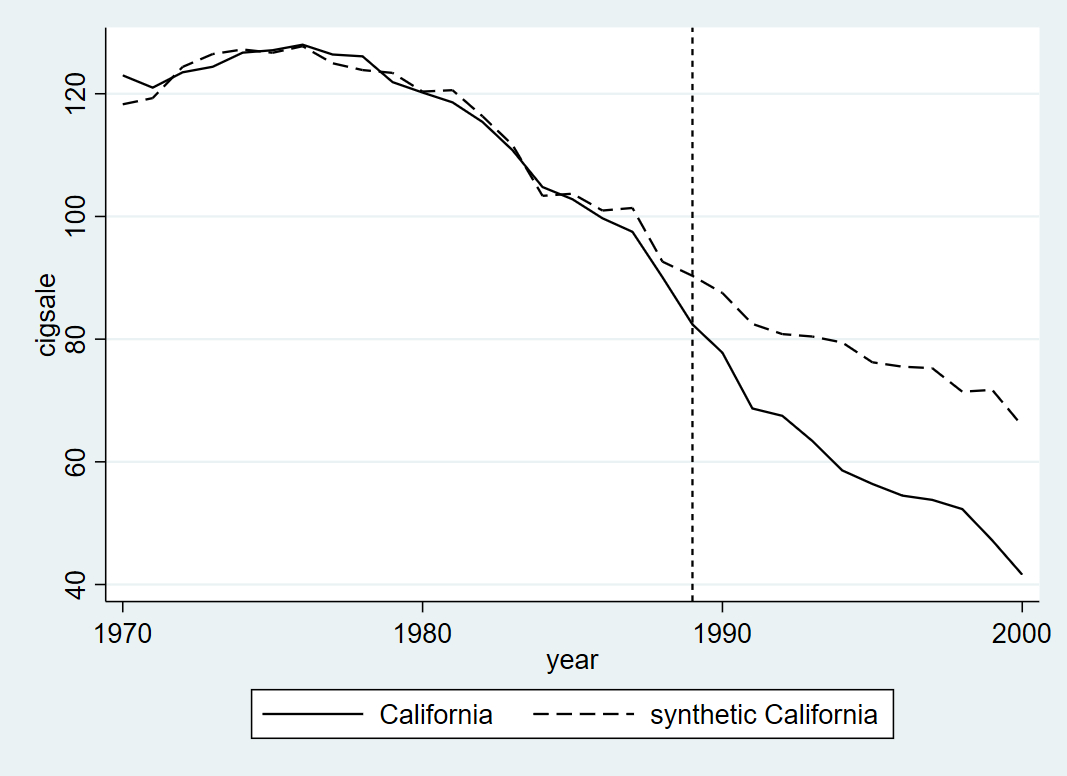
\includegraphics[width=0.9\textwidth]{figure/CA.png}
		\end{figure}
	\end{center}
\end{frame}



\begin{frame}{SC Analysis for Non-treated States}{Alabama}
	\begin{center}
		\begin{figure}[p]
			\centering
			%\scalebox{0.98}{\includegraphics{did_1.jpg}}
			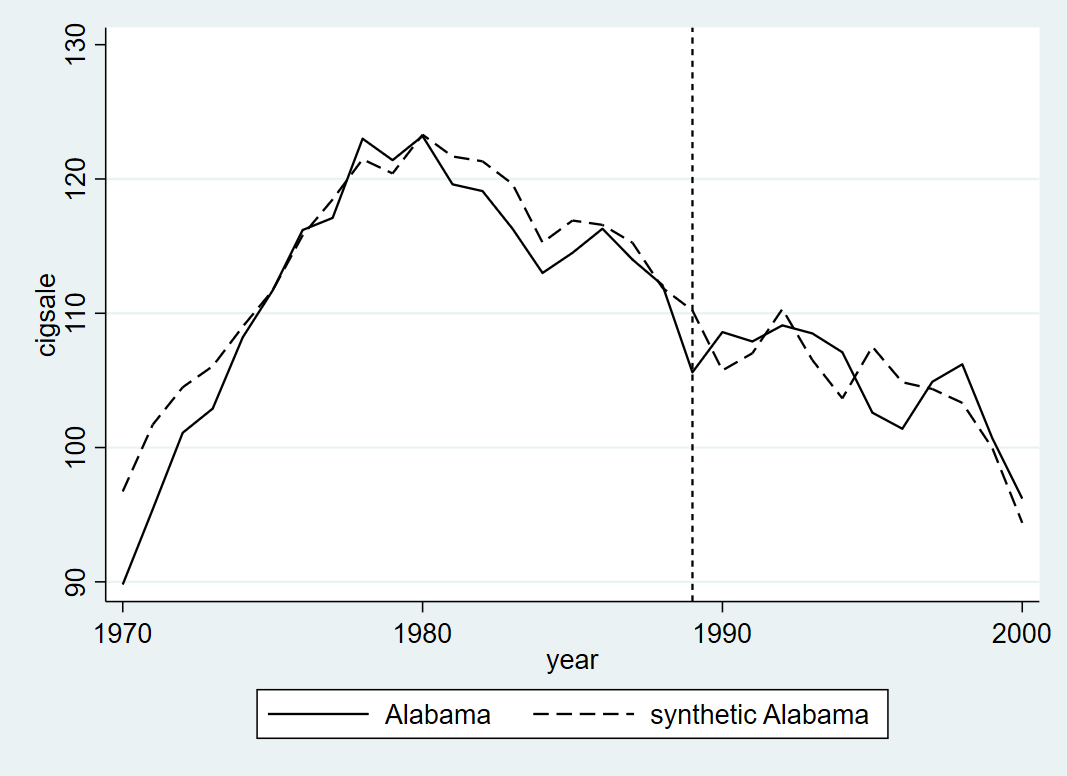
\includegraphics[width=0.9\textwidth]{figure/state1.png}
		\end{figure}
	\end{center}
\end{frame}


\begin{frame}{SC Analysis for Non-treated States}{Arkansas}
	\begin{center}
		\begin{figure}[p]
			\centering
			%\scalebox{0.98}{\includegraphics{did_1.jpg}}
			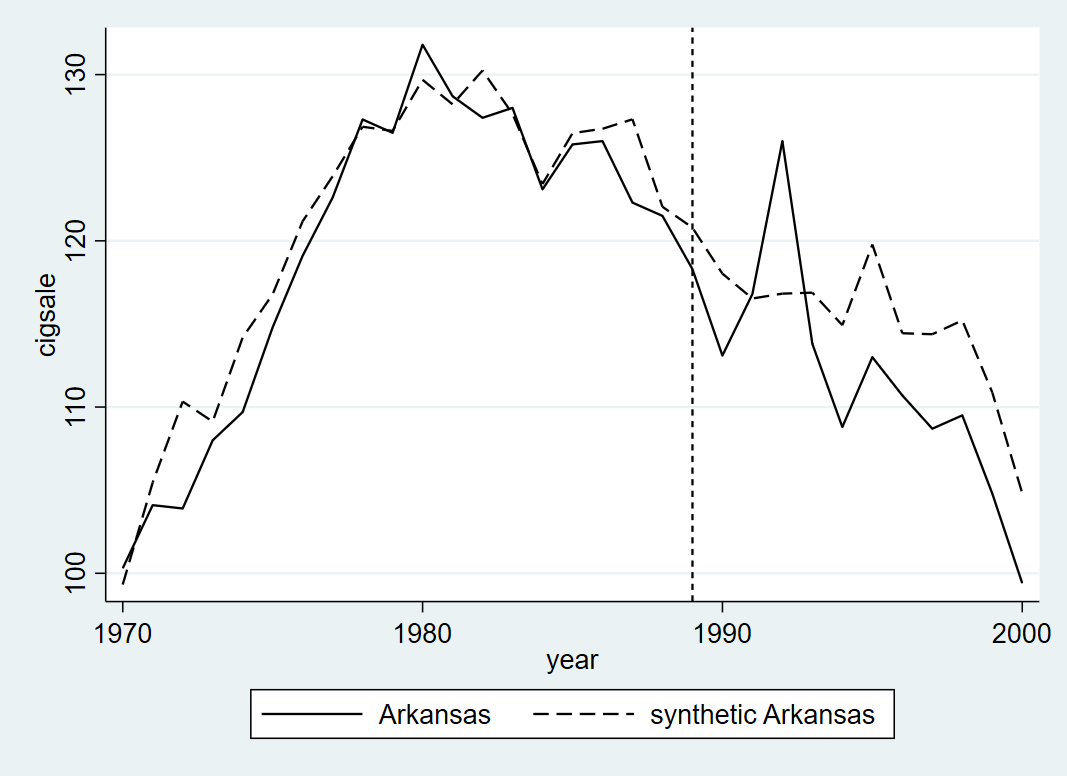
\includegraphics[width=0.9\textwidth]{figure/state2.png}
		\end{figure}
	\end{center}
\end{frame}


\begin{frame}{SC Analysis for Non-treated States}{Colorado}
	\begin{center}
		\begin{figure}[p]
			\centering
			%\scalebox{0.98}{\includegraphics{did_1.jpg}}
		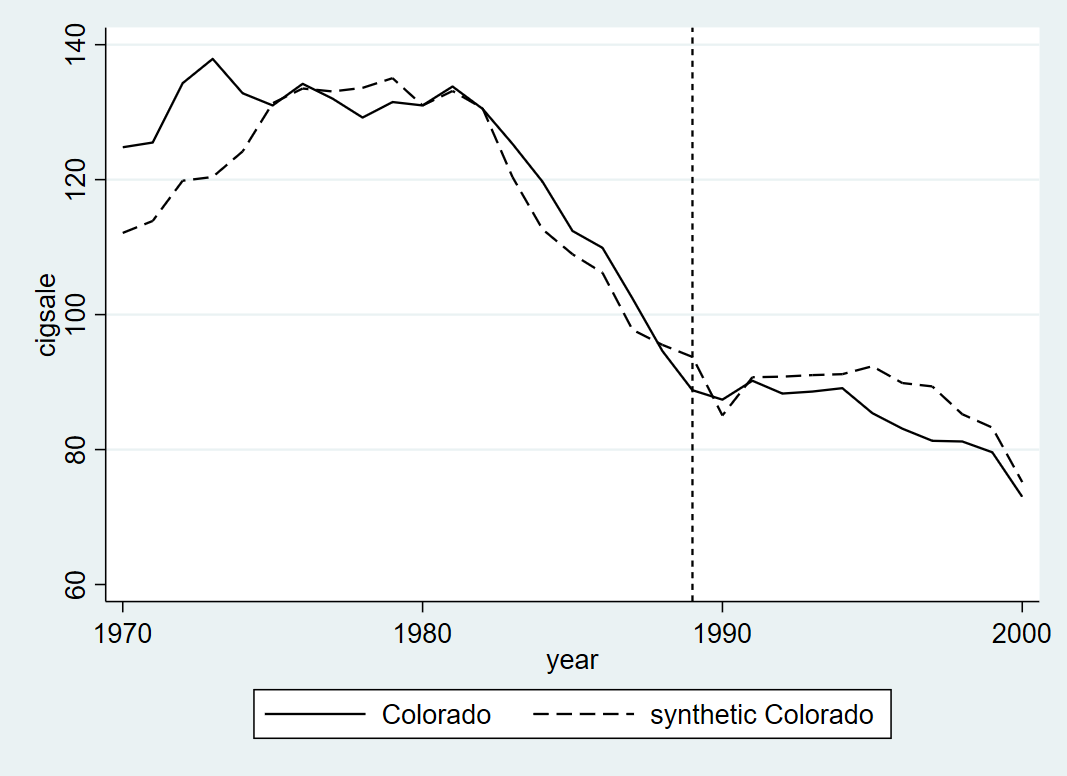
\includegraphics[width=0.9\textwidth]{figure/state4.png}
		\end{figure}
	\end{center}
\end{frame}


\begin{frame}{SC Analysis for Non-treated States}{Connecticut}
	\begin{center}
		\begin{figure}[p]
			\centering
			%\scalebox{0.98}{\includegraphics{did_1.jpg}}
			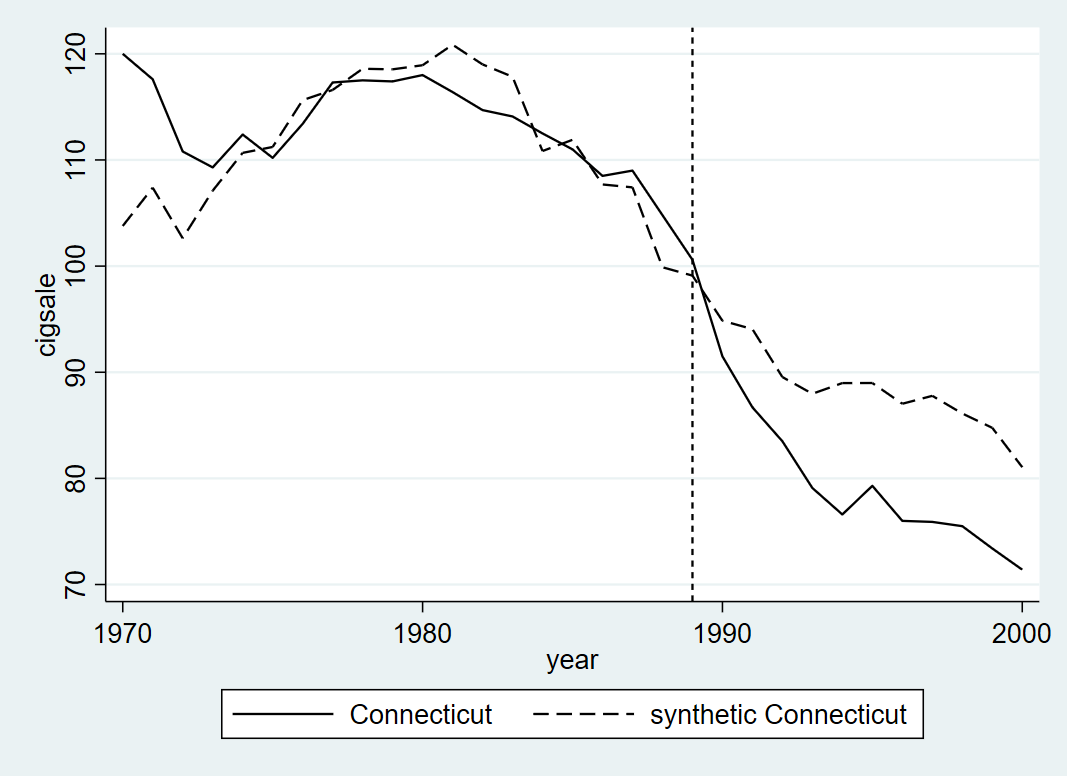
\includegraphics[width=0.9\textwidth]{figure/state5.png}
		\end{figure}
	\end{center}
\end{frame}


\begin{frame}{SC Estimates for California vs. Non-treated States}{Use All Placebo Estimates}
\begin{center}
\begin{figure}[p]
\centering
%\scalebox{0.98}{\includegraphics{did_1.jpg}}
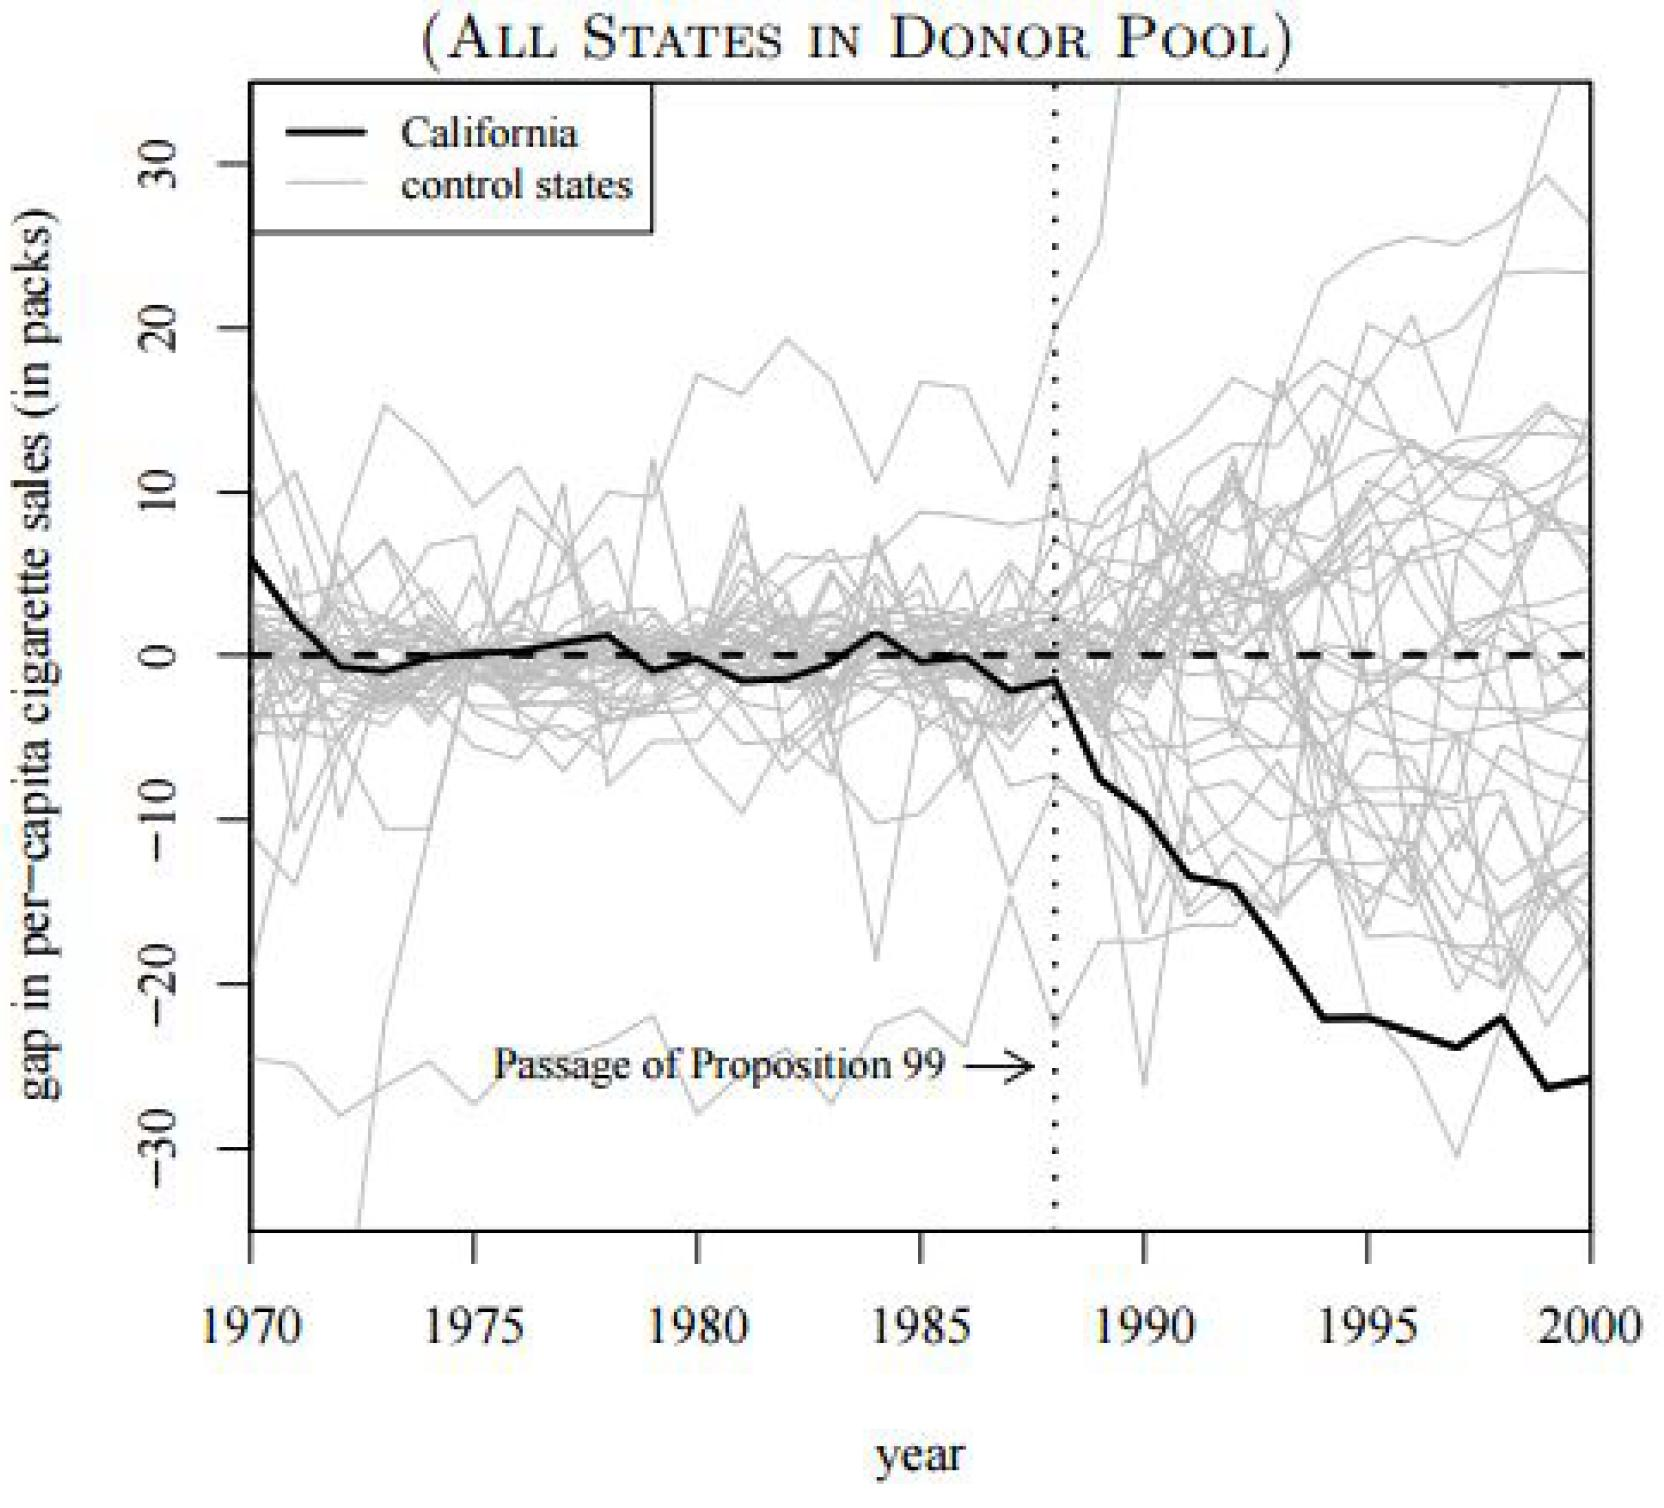
\includegraphics{figure/sc-4.jpg}
\end{figure}
\end{center}
\end{frame}



\begin{frame}{Statistical Inference of SC}
\begin{itemize}
\item The placebo effects may be quite large if those units were NOT matched well in the pre-treatment period
\vspace{0.2cm}
\item For example, when the SC fit is bad, we may get erroneous inferences 
\vspace{0.2cm}
\begin{itemize}
\item Look at bottom gray line in the above figure
\vspace{0.2cm}
\end{itemize}
\item This would cause too large p-values 


\end{itemize}
\end{frame}


\begin{frame}{Statistical Inference of SC}{}
	\begin{itemize}
		\item To control for this, one may want to \textbf{adjust $\hat{\alpha}_{it}$ for the quality of the pre-treatment matches}
		\vspace{0.2cm}
		
		
		\item \textbf{Method 1:}
				\vspace{0.2cm}
			\begin{itemize}
		\item Removing observations with too big Root Mean Squared Predictive Error (RMSPE) during the pre-treatment period
		
		
		\begin{equation*}
			RMSPE^{pre}_{i}= 	\sqrt{\dfrac{			\sum^{T_{0}}_{t=1}(Y_{it} - Y^{SC}_{it})^{2}}{T_{0}}}
\end{equation*}
		
			\end{itemize}
	\end{itemize}
\end{frame}







\begin{frame}{SC Estimates for CA vs. Placebo Treatments}{Use High-Quality Placebo Estimates}
\begin{center}
	\begin{figure}[p]
		\centering
		\scalebox{0.85}{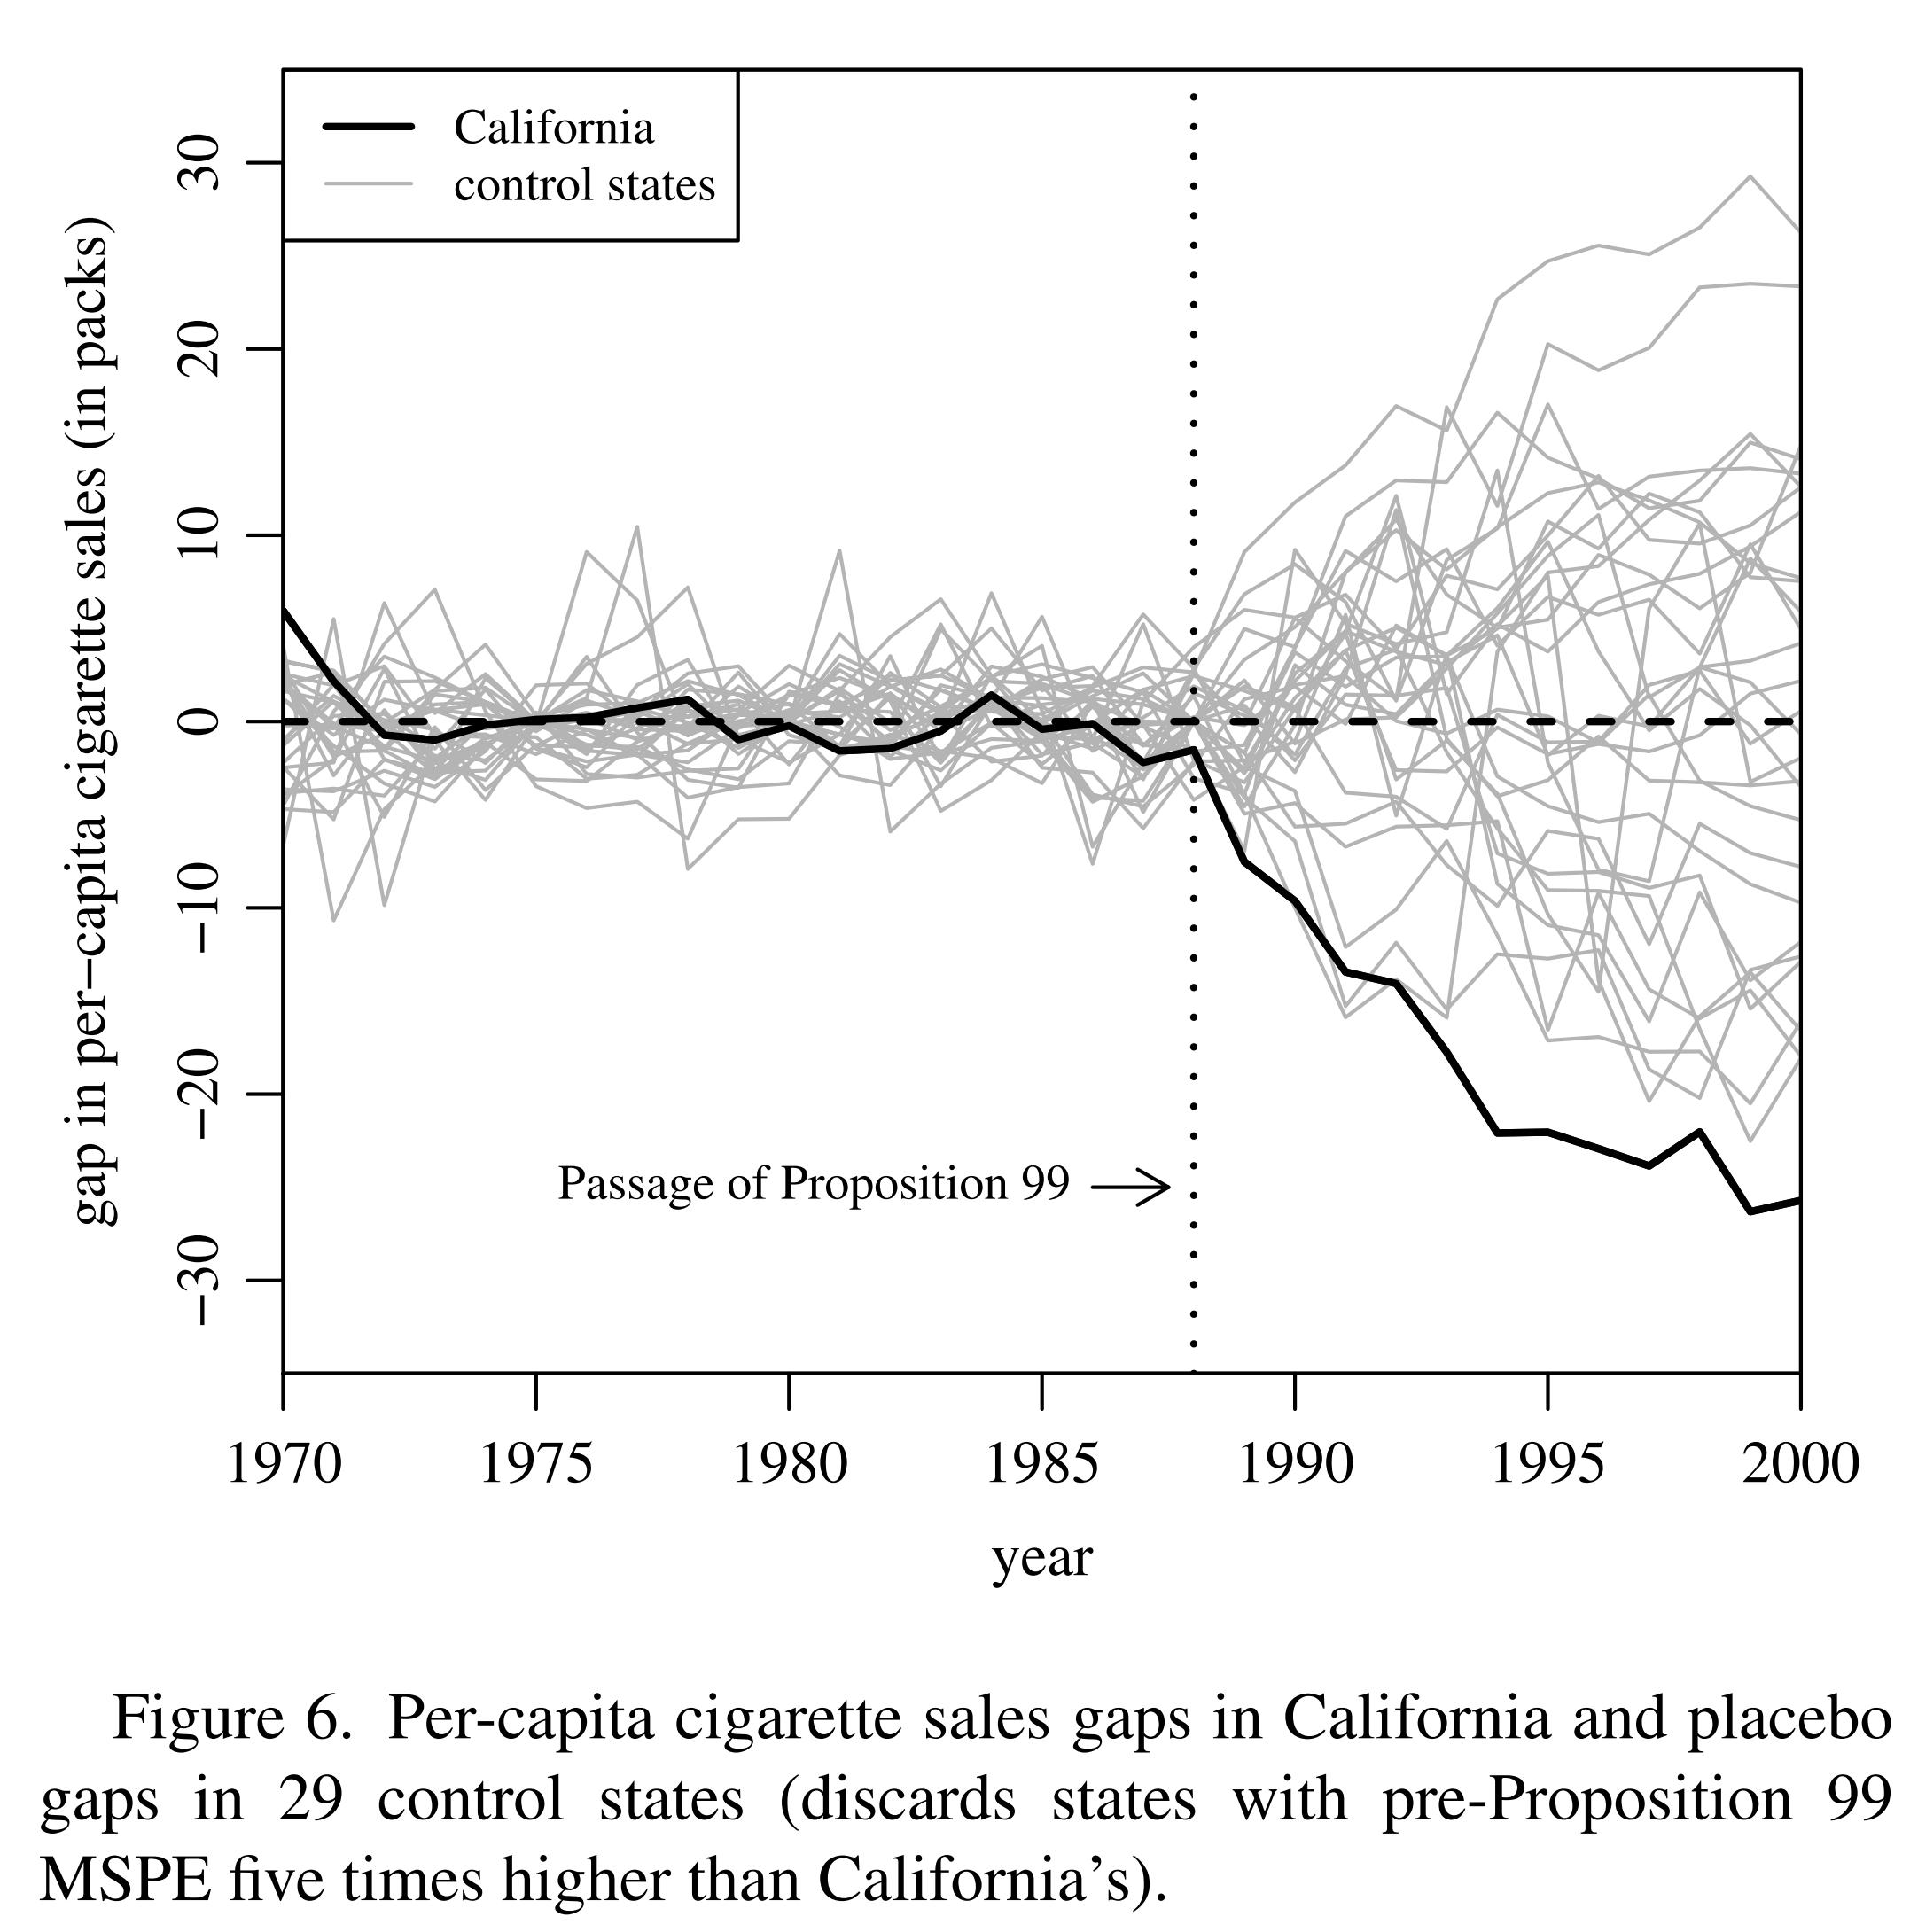
\includegraphics{figure/sc_f6.jpg}}
		%\includegraphics{sc-5.jpg}
	\end{figure}
\end{center}
\end{frame}




\begin{frame}{Statistical Inference of SC}{Standardized p-value}
	\begin{itemize}
		
	\item \textbf{Method 2:}
				\vspace{0.2cm}
			\begin{itemize}
		\item We can also calculate p-value by taking pre-treatment matching quality into account: 
		
	\begin{equation*}
		p^{std}_{1t}=\dfrac{\sum^{J+1}_{i=2}\mathbf{1}\{\dfrac{\hat{\alpha}_{it}}{RMSPE^{pre}_{i}} \geq   \dfrac{\hat{\alpha}_{1t}}{RMSPE^{pre}_{1}}\}}{J}
\end{equation*}
		
		
		\begin{equation*}
			RMSPE^{pre}_{i}= 	\sqrt{\dfrac{			\sum^{T_{0}}_{t=1}(Y_{it} - Y^{SC}_{it})^{2}}{T_{0}}}
\end{equation*}
		
			\end{itemize}
	\end{itemize}
\end{frame}



\begin{frame}{Statistical Inference of SC}{RMSPE Ratio Test}
	\begin{itemize}
		\item \textbf{Method 3:}
		\vspace{0.2cm}
		\begin{itemize}
			\item We can evaluate the significance by comparing the ratio of post/pre-treatment RMSPE:
			
			\begin{equation*}
				p^{ratio}_{1}=\dfrac{\sum^{J+1}_{i=2}\mathbf{1}\{\dfrac{RMSPE^{post}_{i}}{RMSPE^{pre}_{i}} \geq \dfrac{RMSPE^{post}_{1}}{RMSPE^{pre}_{1}}\}}{J}
\end{equation*}
			
			\begin{equation*}
				RMSPE^{post}_{i}= \sqrt{\dfrac{\sum^{T}_{t=T_{0}+1}(Y_{it} - Y^{SC}_{it})^{2}}{T-T_{0}}}
\end{equation*}
			
			\item This method evaluates whether the treatment effect is large relative to the pre-treatment fit
					\vspace{0.2cm}
			\item A large ratio indicates that the post-treatment deviation is substantial compared to pre-treatment matching quality
		\end{itemize}
	\end{itemize}
\end{frame}

\title[]  
{STATA Example}


\author 
{}

%\institute{Institute of Economics, Academia Sinica  \\ Econ, NTU}
%\institute{Institute of Economics, Academia Sinica  \\ IMES/IDAS, NCCU}
\institute{}

%\author 
%{楊子霆 \\ 中研院經濟所}

%\institute 
%{中正大學國際經濟專題研討}




\date
{}


\begin{frame}{}
	\titlepage
\end{frame}


\begin{frame}{STATA Example: Kim (2022)}{The Effect of Paid Leave on Fertility}
Brian Kim (2022), \textbf{``The Effect of Paid Leave on Fertility: Evidence from New York''}, Master Thesis
\begin{itemize}
	\vspace{0.2cm}
	\item The study examines the effect of paid parental leave on fertility rates in New York using synthetic control analysis.
	\vspace{0.2cm}
	\item Synthetic control method is used to estimate the counterfactual fertility rates in the absence of the policy.
\end{itemize}
\end{frame}




\begin{frame}{Overview}{Program and Data}
	\begin{itemize}
		\item See SCM.do
		\vspace{0.2cm}
		\item Use fert\_rate\_synth.csv
		\vspace{0.2cm}
		\item Install the following ado files:
		\begin{itemize}
			\vspace{0.2cm}
			\item synth2.ado 
		
			
		\end{itemize}
		
	\end{itemize}
\end{frame}





\begin{frame}[fragile]{Overview}{Stata Commends}
\begin{itemize}

	\item \texttt{synth2}:
	\vspace{0.2cm}
	\begin{itemize}
		\item Can be used for \textbf{single treated unit}
		\vspace{0.2cm}
		\item Supports \textbf{placebo tests} and allows for the exclusion of control units with poor pre-treatment fit.
		\vspace{0.2cm}
		\item Provides options for \textbf{graphing and post-processing}, including the ability to save and export results as graphs.
		\vspace{0.2cm}
		\item Offers robust options for conducting \textbf{statistical inference}, including the ability to calculate p-values.
	\end{itemize}
\end{itemize}
\end{frame}




\begin{frame}[fragile]{Overview}{Data}	
	\begin{itemize}
		
		
		\item This project examines the effect of paid-parental leave on fertility
					\vspace{0.2cm}		
		\begin{itemize}
			\item New York implements paid-parental leave in 2018
			\vspace{0.2cm}		
		\end{itemize}
		
		\item Use synthetic control method to evaluate its impact		
		\vspace{0.2cm}		
		\item The dataset contains state-level fertility rate and other demographic variables from 2007-2019
		\vspace{0.2cm}
		
		
		\begin{itemize}	
			\vspace{0.2cm}	
			\item \textbf{fert:} Fertility rate, which is the outcome variable
			\vspace{0.2cm}
			\item \textbf{year:} This is the year and is the time variable
			\vspace{0.2cm}
			\item \textbf{state:} This is an id number for each state and provides the individual identifier in this panel data context
		\end{itemize}
		
	\end{itemize}
	
	
	
	
\end{frame}



\begin{frame}[fragile]{Install package}
\begin{lstlisting}
ssc install synth2
\end{lstlisting}
	
\begin{lstlisting}
net install gr_postproduce, from("https://raw.githubusercontent.com/DiegoCiccia/StataPostProduce/main") replace
\end{lstlisting}
	
\begin{itemize}
	\item \texttt{synth2} is used for synthetic control analysis, while \texttt{gr\_postproduce} helps with post-processing and customizing graphs.
\end{itemize}	
\end{frame}






\begin{frame}[fragile]{Step 0: Data Preparation}
\begin{itemize}
	\item Assign labels to states based on their IPUMS codes. This allows us to translate numeric codes into meaningful state names in our analysis:
	\vspace{0.2cm}
\begin{lstlisting}
label define state_labels 1 "Alabama" 2 "Alaska" ...
label values ipums state_labels
\end{lstlisting}
	\item The \texttt{label define} command creates a mapping between the state codes and their names, while \texttt{label values} applies this label to the \texttt{ipums} variable.
	\vspace{0.2cm}
	\item This step ensures that state names are displayed in the results instead of numeric codes, making interpretation easier.
\end{itemize}
\end{frame}





\begin{frame}[fragile]{Step 1: Setting Up Panel Data}
\begin{itemize}
	\item Declare the data as panel data:
\begin{lstlisting}
xtset ipums year
\end{lstlisting}
	\item The \textbf{xtset} command declares \texttt{ipums} as the panel variable (state) and `year` as the time variable.

\end{itemize}
\end{frame}


\begin{frame}[fragile]{Step 2: SC Estimation}
\begin{itemize}
	\item Syntax:	
\begin{lstlisting}
synth2 depvar predictorvars, trunit(#) trperiod(#)
\end{lstlisting}
	
	\item \textbf{depvar}: the outcome variable (Y)
	\vspace{0.2cm}
	\item \textbf{predictorvars}: the list of predictor variables (Z)
	\vspace{0.2cm}
	\item By default, all predictor variables are \textbf{averaged over the entire pre-treatment period}
\end{itemize}


\end{frame}


\begin{frame}[fragile]{Step 2: SC Estimation}
\begin{itemize}
	\item Run the synthetic control method using `synth2`:
\begin{lstlisting}
synth2 fert avginc black educattain white asian_pi hisp ///
fert(2017) fert(2016) fert(2015) fert(2014) fert(2013) fert(2012) ///
fert(2011) fert(2010) fert(2009) fert(2008) fert(2007), ///
trunit(36) trperiod(2018) xperiod(2007(1)2017)
\end{lstlisting}
\vspace{0.2cm}
\item \textbf{fert(2017)}: the value of the variable \textbf{fert} in 2017 is entered as a predictor
\vspace{0.2cm}
\item \textbf{xperiod(2007(1)2017)}: periods over 2007-2017 the covariates specified in predictorvars are averaged
\end{itemize}
\end{frame}


\begin{frame}{Results: Unit Weights for SC}
\begin{itemize}
	\item Top 3 states that constitute the synthetic New York
	\begin{itemize}
		\vspace{0.2cm}
		\item New Hampshire: 23.1\%
		\vspace{0.2cm}
		\item Kansas: 23.1\%
		\vspace{0.2cm}
		\item Massachusetts: 15.8\%		
	\end{itemize}
	
	
\end{itemize}
\end{frame}


\begin{frame}[fragile]{Step 3: Statistical Inference}
\begin{itemize}
\item Conduct placebo tests using the `synth2` command:
\begin{lstlisting}
synth2 fert fert(2017) fert(2016) fert(2015) fert(2014) ///
fert(2013) fert(2012) fert(2011) fert(2010) fert(2009) ///
fert(2008) fert(2007), trunit(36) trperiod(2018) ///
xperiod(2007(1)2017) placebo(unit cutoff(2))
\end{lstlisting}
	\item The \textbf{placebo(unit cutoff(2))} option excludes states where pre-treatment RMSPE is more than twice that of the treated unit (New York).
\end{itemize}
\end{frame}




\begin{frame}[fragile]{Graphing Results}
\begin{itemize}
	\item Generate a data frame for storing results and save graphs:
\begin{lstlisting}
synth2 fert fert(2017) fert(2016) fert(2015) fert(2014) ///
fert(2013) fert(2012) fert(2011) fert(2010) fert(2009) ///
fert(2008) fert(2007), trunit(36) trperiod(2018) ///
xperiod(2007(1)2017) frame(ny_fert) savegraph(ny_fert, replace)
\end{lstlisting}

\end{itemize}
\end{frame}


\begin{frame}[fragile]{Post-Processing Graphs}
\begin{itemize}
	\item Enhance graph appearance:
\vspace{0.2cm}
\begin{lstlisting}
graph use "$pic\ny_fert_eff.gph"

gr_postproduce ny_fert_eff, ///
title("The Effect of Paid Leave on Fertility") ///
ytitle("Effects") xtitle("Year")
graph export "$pic\ny_fert_eff.png"
\end{lstlisting}
\item Post-process and export the graph with \textbf{gr\_postproduce}
\end{itemize}
\end{frame}


\begin{frame}[fragile]{Working with Frames}
\begin{itemize}
	\item Switch to the results frame:
	\vspace{0.2cm}
\begin{lstlisting}
frame change ny_fert
\end{lstlisting}
	\vspace{0.2cm}
	\item Export results to CSV:
	\vspace{0.2cm}
\begin{lstlisting}
export delimited "$rawdata\ny_fert.csv",replace
\end{lstlisting}
	\vspace{0.2cm}
	\item Clear all frames and return to default:
	\vspace{0.2cm}
\begin{lstlisting}
frames reset
\end{lstlisting}
\end{itemize}

\end{frame}



\title[]  
{R Example}


\author 
{}

%\institute{Institute of Economics, Academia Sinica  \\ Econ, NTU}
%\institute{Institute of Economics, Academia Sinica  \\ IMES/IDAS, NCCU}
\institute{}

%\author 
%{楊子霆 \\ 中研院經濟所}

%\institute 
%{中正大學國際經濟專題研討}




\date
{}


\begin{frame}{}
\titlepage
\end{frame}




\begin{frame}{Overview}{Program and Data}
\begin{itemize}
	\item See SCM.R
	\vspace{0.2cm}
	\item Use fert\_rate\_synth.csv
	\vspace{0.2cm}
	\item Install the following package:
	\begin{itemize}
		\vspace{0.2cm}
		\item tidysynth 
		
		
	\end{itemize}
	
\end{itemize}
\end{frame}



\begin{frame}[fragile]{Step 0: Install package}
\begin{itemize}
	\item Install required packages:
	\vspace{0.2cm}
\begin{lstlisting}[language=R, style=r-style]
install.packages("tidysynth")


library(tidyverse)
library(tidysynth)
library(haven)
\end{lstlisting}
	\item \textbf{tidysynth}: Main package for synthetic control
	\item \textbf{tidyverse}: Data manipulation and visualization
	\item \textbf{haven}: Reading various data formats
\end{itemize}
\end{frame}

\begin{frame}[fragile]{Step 0: Data Preparation}
\begin{itemize}
\item Read and clean the data:
\vspace{0.2cm}
\begin{lstlisting}[language=R, style=r-style]
fert_data <- fert_data_raw %>%
# Drop specific states and years
filter(!(ipums %in% c(6, 34, 44, 53))) %>%  
filter(year < 2020) %>%
mutate(
avginc = Personal.income/Population
) %>%
select(-statecode)
\end{lstlisting}
\vspace{0.2cm}
\item Key steps:
\begin{itemize}
	\item Drop CA, NJ, RI, WA (states with similar policies)
	\item Remove data after 2020
	\item Calculate average income
	\item Remove unnecessary columns
\end{itemize}
\end{itemize}
\end{frame}

\begin{frame}[fragile]{Step 2: SC Estimation}
\begin{itemize}
\item Initialize synthetic control:
\vspace{0.2cm}
\begin{lstlisting}[language=R, style=r-style]
synth_fert <- fert_data %>%
synthetic_control(
outcome = fert,
unit = state,
time = year,
i_unit = "New York",
i_time = 2018,
generate_placebos = TRUE
)
\end{lstlisting}
\vspace{0.2cm}
\item Parameters:
\begin{itemize}
\item \texttt{outcome}: Fertility rate
\item \texttt{unit}: State identifier
\item \texttt{i\_unit}: Treated unit (New York)
\item \texttt{i\_time}: Treatment year (2018)
\end{itemize}
\end{itemize}
\end{frame}

\begin{frame}[fragile]{Step 2: SC Estimation}{Add Predictors}
\begin{itemize}
\item Add demographic predictors:
\vspace{0.2cm}
\begin{lstlisting}[language=R, style=r-style]
generate_predictor(
time_window = 2007:2017,
avg_income = mean(avginc, na.rm = TRUE),
black_pop = mean(black, na.rm = TRUE),
educ_attain = mean(educattain, na.rm = TRUE),
white_pop = mean(white, na.rm = TRUE),
asian_pop = mean(asian_pi, na.rm = TRUE),
hisp_pop = mean(hisp, na.rm = TRUE)
)
\end{lstlisting}
\item Takes average of demographics over 2007-2017
\item Handles missing values with \texttt{na.rm = TRUE}
\end{itemize}
\end{frame}

\begin{frame}[fragile]{Step 2: SC Estimation}{Add Predictors}
\begin{itemize}
\item Add lagged fertility rates:
\vspace{0.2cm}
\begin{lstlisting}[language=R, style=r-style]
generate_predictor(
time_window = 2017,
fert_2017 = fert
) %>%
generate_predictor(
time_window = 2016,
fert_2016 = fert
)
# ... (similar for other years)
\end{lstlisting}
\item Adds fertility rates for each year from 2007-2017
\item Each year added separately for flexibility
\end{itemize}
\end{frame}

\begin{frame}[fragile]{Step 2: SC Estimation}{Weight Generation}
\begin{itemize}
\item Generate synthetic control weights:
\vspace{0.2cm}
\begin{lstlisting}[language=R, style=r-style]
 # Generate weights using default optimization parameters
generate_weights(optimization_window = 2007:2017) %>%
generate_control()
\end{lstlisting}
\item Parameters:
\begin{itemize}
\item \texttt{optimization\_window}: Time period for weight calculation
%\item \texttt{margin\_ipop}: Convergence margin
%\item \texttt{sigf\_ipop}: Significant figures in optimization
%\item \texttt{bound\_ipop}: Optimization boundary
\end{itemize}
\end{itemize}
\end{frame}

\begin{frame}[fragile]{Graphing Results}
\begin{itemize}
\item Generate and display plots:
\vspace{0.2cm}
\begin{lstlisting}[language=R, style=r-style]
plot_trends <- synth_fert %>%
plot_trends() +
labs(
title = "Fertility Trends: NY vs Synthetic Control",
y = "Fertility Rate",
x = "Year"
)

print(plot_trends)  
ggsave("synth_fert.png", plot = plot_trends)
\end{lstlisting}
\item Three types of plots:
\begin{itemize}
\item Trends plot: Actual vs synthetic
\item Differences plot: Gap analysis
\item Placebos plot: Statistical inference
\end{itemize}
\end{itemize}
\end{frame}


\begin{frame}[fragile]{Graphing Results}
\begin{itemize}
	\item Generate and display difference plot:
	\vspace{0.2cm}
\begin{lstlisting}[language=R, style=r-style]
plot_differences <- synth_fert %>%
plot_differences() +
labs(
title = "Gap in Fertility Rates",
y = "Difference in Fertility Rate",
x = "Year"
)

print(plot_differences)
ggsave("synth_fert_differences.png", 
plot = plot_differences)
\end{lstlisting}
	\item Gap Analysis Features:
	\begin{itemize}
		\item Shows treatment effect over time
		\item Zero line indicates no effect
		\item Negative values show fertility decrease
		\item Helps identify pre-treatment fit quality
	\end{itemize}
\end{itemize}
\end{frame}

\begin{frame}[fragile]{Graphing Results}
\begin{itemize}
\item Generate and display placebo plot:
\vspace{0.2cm}
\begin{lstlisting}[language=R, style=r-style]
plot_placebos <- synth_fert %>%
plot_placebos() +
labs(
title = "Placebo Tests",
y = "Gap in Fertility Rate",
x = "Year"
)

print(plot_placebos)
ggsave("synth_fert_placebos.png", 
plot = plot_placebos)
\end{lstlisting}
\item Placebo Test Features:
\begin{itemize}
	\item Shows treatment effects for all states
	\item Treated unit highlighted
	\item Provides visual inference
	\item Helps assess significance of results
\end{itemize}
\end{itemize}
\end{frame}

\begin{frame}[fragile]{Results Export}
\begin{itemize}
\item Save results and tables:
\vspace{0.2cm}
\begin{lstlisting}[language=R, style=r-style]
summary_tables <- synth_fert %>%
grab_synthetic_control()
predictor_balance <- synth_fert %>%
grab_balance_table()


write_csv(summary_tables, 
file.path(workdata, "ny_fert_results.csv"))
write_csv(predictor_balance, 
file.path(workdata, "ny_fert_balance.csv"))
\end{lstlisting}
\item Exports:
\begin{itemize}
\item Synthetic control results
\item Predictor balance tables
\end{itemize}
\end{itemize}
\end{frame}













\begin{comment}
% ============================================================
\title[]{Recent Development}
\author{}
\institute{}
\date{}

\begin{frame}{}
	\titlepage
\end{frame}


\begin{frame}{Recent Developments}{Overview}
\begin{itemize}
	\item Standard SC method (Abadie et al., 2010) was designed for a \textbf{single treated unit}
	\vspace{0.1cm}
	\item Three important recent extensions:
	\vspace{0.1cm}
	\begin{itemize}
		\item[1.] \textbf{Multiple Treated Units}
		\vspace{0.05cm}
		\begin{itemize}
			\item Problem: \textbf{interpolation bias} when many treated units exist
			\item Solution: Abadie \& L'Hour (2019)
		\end{itemize}
		\vspace{0.1cm}
		\item[2.] \textbf{Regression-Based Methods}
		\vspace{0.05cm}
		\begin{itemize}
			\item Problem: standard SC restricts weights to be non-negative and sum to one
			\item Solution: Doudchenko \& Imbens (2016)
		\end{itemize}
		\vspace{0.1cm}
		\item[3.] \textbf{Prediction Intervals}
		\vspace{0.05cm}
		\begin{itemize}
			\item Problem: permutation tests do not quantify estimation uncertainty directly
			\item Solution: Cattaneo et al.\ (2021)
		\end{itemize}
	\end{itemize}
\end{itemize}
\end{frame}


\begin{frame}{Multiple Treated Units}{Basic Setup}
\begin{itemize}
	\item Now suppose there are $I$ treated units ($i=1,\ldots,I$) and $J$ untreated (donor) units ($j=I+1,\ldots,I+J$)
	\vspace{0.2cm}
	\item \textbf{No conceptual problem}: construct a separate synthetic control for each treated unit $i$
	\vspace{0.2cm}
	\begin{itemize}
		\item Individual treatment effect for unit $i$ at time $t > T_0$:
		\begin{equation*}
			\hat{\tau}_{it} = Y_{it} - \sum_{j=I+1}^{I+J} w_{ij}^{*}\,Y_{jt}
		\end{equation*}
		\vspace{0.1cm}
		\item Average treatment effect across all treated units:
		\begin{equation*}
			\hat{\tau}_{t} = \frac{1}{I}\sum_{i=1}^{I}\hat{\tau}_{it}
		\end{equation*}
	\end{itemize}
	\vspace{0.2cm}
	\item \textbf{Practical challenge}: having many treated units makes choosing the optimal weights harder due to \textbf{interpolation bias}
\end{itemize}
\end{frame}


\begin{frame}{Multiple Treated Units}{Interpolation Bias}
\begin{itemize}
	\item \textbf{Convex hull}: the smallest convex set that contains all donor units $\{X_{I+1},\ldots,X_{I+J}\}$
	\vspace{0.2cm}
	\item If $X_i$ lies \textbf{inside} the convex hull of the donor pool, there may be \textbf{infinitely many} feasible $W_i$ such that $X_i = X_0 W_i$
	\vspace{0.2cm}
	\begin{itemize}
		\item Perfect pre-treatment fit does \textbf{not} uniquely pin down the weights
		\vspace{0.2cm}
		\item \textbf{Interpolation bias}: among the many feasible $W_i$'s, some place large weights on donor units \textbf{far from} unit $i$, producing a poor counterfactual even with perfect fit
	\end{itemize}
	\vspace{0.2cm}
	\item With a \textbf{single} treated unit: non-uniqueness is rare; trimming the donor pool usually resolves it
	\vspace{0.2cm}
	\item With \textbf{many} treated units: choosing among many feasible $W_i$'s becomes a central estimation problem
\end{itemize}
\end{frame}


\begin{frame}{Multiple Treated Units}{Abadie \& L\'Hour (2019): Penalized Estimator}
\begin{itemize}
	\item Propose a \textbf{penalized} SC objective that discourages relying on distant donors
	\vspace{0.1cm}
	\item For each treated unit $i$, minimize:
	\begin{equation*}
		\|X_i - X_0 W_i\|^2
		\;+\;
		\lambda\sum_{j=I+1}^{I+J} w_{ij}\,\|X_i - X_j\|^2
	\end{equation*}
	subject to $w_{ij}\geq 0$ and $\sum_j w_{ij}=1$
	\vspace{0.2cm}
	\item \textbf{First term}: standard SC --- minimize mismatch in predictors $X$ between unit $i$ and its synthetic control
	\vspace{0.2cm}
	\item \textbf{Second term} (penalty): each donor $j$ is penalized by its \textbf{distance} $\|X_i - X_j\|^2$ from treated unit $i$
	\vspace{0.2cm}
	\begin{itemize}
		\item A distant donor contributes more to the penalty $\Rightarrow$ receives a smaller weight
	\end{itemize}
	\vspace{0.2cm}
	\item $\lambda \geq 0$ governs the trade-off: larger $\lambda$ places more emphasis on using \textbf{nearby} donors
\end{itemize}
\end{frame}


\begin{frame}{Multiple Treated Units}{Abadie \& L\'Hour (2019): Properties}
\begin{itemize}
	\item \textbf{Why does the penalty resolve the non-uniqueness problem?}
	\vspace{0.2cm}
	\begin{itemize}
		\item When $\lambda=0$: standard SC; solution may be \textbf{non-unique} if $X_i$ is in the interior of the convex hull
		\vspace{0.2cm}
		\item When $\lambda>0$: among all weight vectors with equally good aggregate fit, the penalty selects the one using \textbf{closer} donors --- the solution becomes \textbf{unique}
	\end{itemize}
	\vspace{0.2cm}
	\item \textbf{Key properties:}
	\vspace{0.2cm}
	\begin{itemize}
		\item \textbf{Unique solution} when $\lambda>0$ --- interpolation bias is reduced
		\vspace{0.2cm}
		\item \textbf{Sparsity}: only a few nearby donors receive positive weights, making the synthetic control transparent and interpretable
	\end{itemize}
\end{itemize}
\end{frame}


\begin{frame}{Regression-Based Synthetic Control}{Motivation}
\begin{itemize}
	\item Standard SC constrains the weights:
	\begin{equation*}
		w_i \geq 0
		\quad\text{and}\quad
		\sum_{i=2}^{J+1} w_i = 1
	\end{equation*}
	\vspace{0.1cm}
	\item These constraints ensure \textbf{no extrapolation}: the synthetic unit always lies \textbf{within} the convex hull of the donor pool
	\vspace{0.2cm}
	\item \textbf{Problem:} if the treated unit $X_1$ lies \textbf{outside} the convex hull, perfect pre-treatment fit is impossible
	\vspace{0.2cm}
	\begin{itemize}
		\item The synthetic unit cannot fully match the treated unit's trajectory
		\vspace{0.2cm}
		\item Residual pre-treatment mismatch may bias post-treatment estimates
	\end{itemize}
	\vspace{0.2cm}
	\item \textbf{Idea:} relax the non-negativity and summation constraints to allow \textbf{extrapolation}
\end{itemize}
\end{frame}


\begin{frame}{Regression-Based Synthetic Control}{Doudchenko \& Imbens (2016)}
\begin{itemize}
	\item Estimate the counterfactual with an \textbf{intercept} and \textbf{unconstrained} weights:
	\begin{equation*}
		\hat{Y}^{0}_{1t} = \hat{\alpha} + \sum_{j=2}^{J+1} \hat{w}_j\,Y_{jt},
		\quad t > T_0
	\end{equation*}
	\item Choose parameters $(\alpha, w_2, \ldots, w_{J+1})$ to minimize an \textbf{elastic-net} penalized pre-treatment loss:
	\begin{equation*}
		\sum_{t=1}^{T_0}\!\left(Y_{1t} - \alpha - \sum_{j=2}^{J+1}w_j Y_{jt}\right)^{\!2}
		+\,\lambda_1\!\left(\frac{1-\lambda_2}{2}\sum_j w_j^2
		+\,\lambda_2\sum_j|w_j|\right)
	\end{equation*}
	\vspace{0.1cm}
	\item \textbf{Features:}
	\vspace{0.1cm}
	\begin{itemize}
		\item Weights may be \textbf{negative} and need \textbf{not sum to one} --- extrapolation allowed
		\vspace{0.1cm}
		\item $\hat{\alpha}$ absorbs a constant level difference between treated and donors
		\vspace{0.1cm}
		\item Regularization combines \textbf{ridge} ($\lambda_2=0$, shrinks all weights) and \textbf{lasso} ($\lambda_2=1$, produces sparse weights)
		\vspace{0.1cm}
		\item Trade-off: more flexible fit, but higher variance --- requires careful choice of $\lambda_1, \lambda_2$
	\end{itemize}
\end{itemize}
\end{frame}


% -------------------------------------------------------------------
\begin{frame}{Prediction Intervals in SC}{Motivation}
\begin{itemize}
	\item So far, statistical inference in SC relies on \textbf{permutation (placebo) tests}
	\vspace{0.3cm}
	\item Permutation tests answer: ``Is the estimated treatment effect \textbf{unusually large} compared to placebo units?''
	\vspace{0.3cm}
	\item But they do \textbf{not} directly tell us:
	\vspace{0.2cm}
	\begin{itemize}
		\item How uncertain is our estimate $\hat{\alpha}_{1t}$ of the true effect $\alpha_{1t}$?
		\vspace{0.2cm}
		\item What is the plausible \textbf{range} of the true treatment effect?
	\end{itemize}
	\vspace{0.3cm}
	\item \textbf{Prediction intervals} (Cattaneo et al., 2021) fill this gap by constructing a confidence band around $\hat{\alpha}_{1t}$ for each post-treatment period $t$
\end{itemize}
\end{frame}


\begin{frame}{Prediction Intervals in SC}{Two Sources of Uncertainty}
\begin{itemize}
	\item Why is $\hat{\alpha}_{1t}$ not exactly equal to $\alpha_{1t}$? There are \textbf{two reasons}:
	\vspace{0.3cm}
	\item \textbf{Source 1 --- In-sample uncertainty} (weight estimation error)
	\vspace{0.1cm}
	\begin{itemize}
		\item We estimate the weights $\hat{w}_i$ from \textit{pre-treatment} data
		\item They are close to, but not exactly, the ``true'' weights $w_i^0$
		\item This error \textbf{shrinks} as the pre-treatment period $T_0$ grows longer
	\end{itemize}
	\vspace{0.3cm}
	\item \textbf{Source 2 --- Out-of-sample uncertainty} (post-treatment shocks)
	\vspace{0.1cm}
	\begin{itemize}
		\item Even with \textit{perfect} weights, unexpected shocks $e_t$ hit after treatment
		\item The synthetic unit is a \textit{prediction}, not an exact mirror, of the counterfactual
		\item This uncertainty \textbf{cannot} be reduced by having more pre-treatment data
	\end{itemize}
\end{itemize}
\end{frame}


\begin{frame}{Prediction Intervals in SC}{Why Two Sources Matter}
\begin{itemize}
	\item The estimation error decomposes as:
	\begin{equation*}
		\underbrace{\hat{\alpha}_{1t} - \alpha_{1t}}_{\text{estimation error}}
		\;=\;
		\underbrace{-\sum_{i=2}^{J+1}(\hat{w}_i - w_i^0)\,Y_{it}}_{\text{Source 1: in-sample}}
		\;+\;
		\underbrace{e_t}_{\text{Source 2: out-of-sample}}
	\end{equation*}
	\vspace{0.2cm}
	\item \textbf{Intuition for each term:}
	\vspace{0.2cm}
	\begin{itemize}
		\item \textbf{Source 1}: if estimated weights $\hat{w}_i$ deviate from $w_i^0$, the synthetic unit is built from slightly the ``wrong'' mix of donors $\Rightarrow$ introduces bias in post-treatment period
		\vspace{0.2cm}
		\item \textbf{Source 2}: after treatment, the real world experiences shocks that the pre-treatment model did not see $\Rightarrow$ even the best synthetic control will miss
	\end{itemize}
	\vspace{0.2cm}
	\item Traditional permutation tests effectively capture neither source cleanly; prediction intervals account for \textbf{both}
\end{itemize}
\end{frame}


\begin{frame}{Prediction Intervals in SC}{Intuition for Width of Intervals}
\begin{itemize}
	\item The prediction interval is wider when:
	\vspace{0.3cm}
	\begin{itemize}
		\item \textbf{Pre-treatment period is short} ($T_0$ small)
		\vspace{0.1cm}
		\begin{itemize}
			\item Weights $\hat{w}_i$ are estimated with less data $\Rightarrow$ more in-sample uncertainty
		\end{itemize}
		\vspace{0.3cm}
		\item \textbf{Post-treatment shocks are large}
		\vspace{0.1cm}
		\begin{itemize}
			\item Large $e_t$ after treatment $\Rightarrow$ more out-of-sample uncertainty
		\end{itemize}
		\vspace{0.3cm}
		\item \textbf{Pre-treatment fit is poor}
		\vspace{0.1cm}
		\begin{itemize}
			\item Suggests that donor units do not closely track the treated unit $\Rightarrow$ both sources of error are larger
		\end{itemize}
	\end{itemize}
	\vspace{0.3cm}
	\item \textbf{Key message}: good pre-treatment fit is necessary but not sufficient --- post-treatment shocks always remain
\end{itemize}
\end{frame}


\begin{frame}{Prediction Intervals in SC}{Implementation}
\begin{itemize}
	\item Cattaneo et al.\ (2021) develop formal prediction intervals for $\alpha_{1t}$ that account for both in-sample and out-of-sample uncertainty
	\vspace{0.3cm}
	\item Available in the \texttt{scpi} package in R (and Python/Stata)
	\vspace{0.3cm}
	\item The output provides, for each post-treatment period $t$:
	\vspace{0.2cm}
	\begin{itemize}
		\item Point estimate $\hat{\alpha}_{1t}$
		\vspace{0.2cm}
		\item Prediction interval $[\hat{\alpha}_{1t} - \text{margin}_t,\;\hat{\alpha}_{1t} + \text{margin}_t]$
	\end{itemize}
	\vspace{0.3cm}
	\item Can handle both single and multiple treated units
\end{itemize}
\end{frame}



% ==================================================================
%  Stata Example: Recent Developments  (scpi package)
% ==================================================================

\title[]{Stata Example: Recent Developments}
\author{}
\institute{}
\date{}

\begin{frame}{}
\titlepage
\end{frame}


\begin{frame}[fragile]{Install Package}{scpi}
\begin{itemize}
    \item The \texttt{scpi} package (Cattaneo et al.) unifies all three recent extensions in a single framework
    \vspace{0.2cm}
\begin{lstlisting}[language=Stata, style=stata-editor]
net install scpi, replace ///
  from("https://raw.githubusercontent.com/" ///
       "nppackages/scpi/master/stata")
\end{lstlisting}
    \vspace{0.2cm}
    \item Key commands:
    \vspace{0.1cm}
    \begin{itemize}
        \item \texttt{scdata} / \texttt{scdataMulti} --- prepare single / multiple treated unit data
        \vspace{0.1cm}
        \item \texttt{scest} --- point estimation (constraint set via \texttt{name()})
        \vspace{0.1cm}
        \item \texttt{scpi} --- point estimate + prediction intervals
        \vspace{0.1cm}
        \item \texttt{scplot} / \texttt{scplotMulti} --- plot results
    \end{itemize}
\end{itemize}
\end{frame}


\begin{frame}[fragile]{Step 0: Data Preparation}{scdata (Stata)}
\begin{itemize}
    \item \texttt{scpi} requires string unit IDs; decode the numeric \texttt{ipums} variable first
    \vspace{0.2cm}
\begin{lstlisting}[language=Stata, style=stata-editor]
decode ipums, gen(state_str)
drop if state_str == "D.C."

scdata fert, dfname(df_si)            ///
    id(state_str) time(year)          ///
    outcome(fert) unittr("New York")  ///
    period_pre(2007 2017)             ///
    period_post(2018 2019)
\end{lstlisting}
    \vspace{0.2cm}
    \item \texttt{dfname(df\_si)} stores the prepared data object for subsequent \texttt{scest} / \texttt{scpi} calls
\end{itemize}
\end{frame}


\begin{frame}[fragile]{Step 1: Standard SC}{scest --- simplex (Stata)}
\begin{itemize}
    \item Baseline: non-negative weights that sum to one
    \vspace{0.2cm}
\begin{lstlisting}[language=Stata, style=stata-editor]
scest df_si, name(simplex)
scest_display
\end{lstlisting}
    \vspace{0.3cm}
    \item \texttt{name(simplex)}: enforces $w_i \geq 0$ and $\sum_i w_i = 1$
    \vspace{0.2cm}
    \item Replicates the standard Abadie et al.\ (2010) estimator within the \texttt{scpi} framework
\end{itemize}
\end{frame}


\begin{frame}[fragile]{Step 2: Penalized SC}{Abadie \& L'Hour (2019) spirit (Stata)}
\begin{itemize}
    \item Add an L1 (lasso) or L2 (ridge) penalty to the weight objective
    \vspace{0.2cm}
\begin{lstlisting}[language=Stata, style=stata-editor]
* lasso: L1 penalty -- sparse weights, fewer donors
scest df_si, name(lasso)
scest_display

* ridge: L2 penalty -- smooth shrinkage across all donors
scest df_si, name(ridge)
scest_display
\end{lstlisting}
    \vspace{0.2cm}
    \item \texttt{lasso} promotes sparsity and a unique solution (reduces interpolation bias)
    \vspace{0.1cm}
    \item \texttt{ridge} shrinks all weights smoothly toward zero
\end{itemize}
\end{frame}


\begin{frame}[fragile]{Step 3: Regression-Based SC}{Doudchenko \& Imbens (2016) spirit (Stata)}
\begin{itemize}
    \item Remove non-negativity and sum-to-one constraints; freely estimate an intercept
    \vspace{0.2cm}
\begin{lstlisting}[language=Stata, style=stata-editor]
* ols: unconstrained -- weights can be negative
scest df_si, name(ols)
scest_display
\end{lstlisting}
    \vspace{0.3cm}
    \item Useful when the treated unit lies \textbf{outside} the convex hull of donors
    \vspace{0.2cm}
    \item Trade-off: more flexible, but extrapolation may reduce interpretability
\end{itemize}
\end{frame}


\begin{frame}[fragile]{Step 4: Prediction Intervals}{scpi (Stata)}
\begin{itemize}
    \item \texttt{scpi} computes formal prediction intervals accounting for both in-sample and out-of-sample uncertainty
    \vspace{0.2cm}
\begin{lstlisting}[language=Stata, style=stata-editor]
scpi df_si, name(simplex)      ///
    u_order(1) u_lags(0)       ///
    u_sigma(HC1) sims(200)     ///
    e_order(1)  e_lags(0)      ///
    e_method(gaussian)         ///
    u_alpha(0.05) e_alpha(0.05)
scpi_display
\end{lstlisting}
    \vspace{0.2cm}
    \item \texttt{u\_*} models in-sample (weight estimation) uncertainty; \texttt{e\_*} models out-of-sample (post-treatment shock) uncertainty
\end{itemize}
\end{frame}


\begin{frame}[fragile]{Step 4: Prediction Intervals}{Plot (Stata)}
\begin{lstlisting}[language=Stata, style=stata-editor]
cd "$figure"
scplot, name(ny_fert_scpi) format(png) eout
\end{lstlisting}
\begin{itemize}
    \vspace{0.4cm}
    \item \texttt{eout} overlays the prediction interval band on the plot
    \vspace{0.2cm}
    \item The shaded region shows where the treated unit would plausibly fall in the absence of treatment, given both sources of uncertainty
\end{itemize}
\end{frame}


\begin{frame}[fragile]{Step 5: Multiple Treated Units}{scdataMulti (Stata)}
\begin{itemize}
    \item When multiple units receive treatment, use \texttt{scdataMulti} with a 0/1 treatment indicator column
    \vspace{0.2cm}
\begin{lstlisting}[language=Stata, style=stata-editor]
* NY (2018) + Connecticut (2018) as second treated unit
gen treatment = 0
replace treatment = 1 ///
    if state_str == "New York"    & year >= 2018
replace treatment = 1 ///
    if state_str == "Connecticut" & year >= 2018

scdataMulti fert, dfname(df_multi)      ///
    id(state_str) time(year)            ///
    outcome(fert) treatment(treatment)  ///
    period_pre(2007 2017) period_post(2018 2019)
\end{lstlisting}
\end{itemize}
\end{frame}


\begin{frame}[fragile]{Step 5: Multiple Treated Units}{Estimation and Plot (Stata)}
\begin{lstlisting}[language=Stata, style=stata-editor]
* Point estimates -- one synthetic control per treated unit
scest df_multi, name(simplex)
scplotMulti

* With prediction intervals
scpi df_multi, name(simplex)       ///
    u_order(1) u_lags(0)           ///
    u_sigma(HC1) sims(200)         ///
    e_order(1)  e_lags(0)          ///
    e_method(gaussian)             ///
    u_alpha(0.05) e_alpha(0.05)
scplotMulti, type(series)
\end{lstlisting}
\begin{itemize}
    \vspace{0.1cm}
    \item \texttt{type(series)} plots each treated unit separately with its prediction interval
\end{itemize}
\end{frame}


% ==================================================================
%  R Example: Recent Developments  (scpi package)
% ==================================================================

\title[]{R Example: Recent Developments}
\author{}
\institute{}
\date{}

\begin{frame}{}
\titlepage
\end{frame}


\begin{frame}[fragile]{Install Package}{scpi (R)}
\begin{itemize}
    \item Install and load the \texttt{scpi} package
    \vspace{0.2cm}
\begin{lstlisting}[language=R, style=r-style]
install.packages("scpi")
library(scpi)
\end{lstlisting}
    \vspace{0.2cm}
    \item Key functions (parallel to Stata commands):
    \vspace{0.1cm}
    \begin{itemize}
        \item \texttt{scdata()} / \texttt{scdataMulti()} --- data preparation
        \vspace{0.1cm}
        \item \texttt{scest()} --- point estimation
        \vspace{0.1cm}
        \item \texttt{scpi()} --- point estimate + prediction intervals
        \vspace{0.1cm}
        \item \texttt{scplot()} / \texttt{scplotMulti()} --- visualization
    \end{itemize}
\end{itemize}
\end{frame}


\begin{frame}[fragile]{Step 0: Data Preparation}{scdata() (R)}
\begin{lstlisting}[language=R, style=r-style]
donors <- setdiff(unique(fert_data$state),
                  "New York")

df <- scdata(
  df           = fert_data,
  id.var       = "state",
  time.var     = "year",
  outcome.var  = "fert",
  period.pre   = 2007:2017,
  period.post  = 2018:2019,
  unit.tr      = "New York",
  unit.co      = donors,
  cointegrated.data = TRUE
)
\end{lstlisting}
\begin{itemize}
    \vspace{0.1cm}
    \item \texttt{cointegrated.data = TRUE}: assumes a long-run linear relationship between the treated unit and donors in the pre-period
\end{itemize}
\end{frame}


\begin{frame}[fragile]{Step 1: Standard SC}{scest() --- simplex (R)}
\begin{lstlisting}[language=R, style=r-style]
est.simplex <- scest(data = df,
               w.constr = list(name = "simplex"))
summary(est.simplex)
\end{lstlisting}
\begin{itemize}
    \vspace{0.3cm}
    \item \texttt{w.constr = list(name = "simplex")}: $w_i \geq 0$, $\sum_i w_i = 1$
    \vspace{0.2cm}
    \item Replicates the classic Abadie et al.\ (2010) estimator
    \vspace{0.2cm}
    \item \texttt{summary()} reports estimated weights and pre-treatment fit statistics
\end{itemize}
\end{frame}


\begin{frame}[fragile]{Step 2: Penalized SC}{Abadie \& L'Hour (2019) spirit (R)}
\begin{lstlisting}[language=R, style=r-style]
# lasso: L1 penalty -- sparse, fewer donors
est.lasso <- scest(data = df,
               w.constr = list(name = "lasso"))

# ridge: L2 penalty -- smooth shrinkage
est.ridge <- scest(data = df,
               w.constr = list(name = "ridge"))

summary(est.lasso)
summary(est.ridge)
\end{lstlisting}
\begin{itemize}
    \vspace{0.2cm}
    \item \texttt{lasso}: only a few donors receive non-zero weight $\rightarrow$ reduces interpolation bias
    \vspace{0.1cm}
    \item \texttt{ridge}: all donors receive some weight, shrunk toward zero
\end{itemize}
\end{frame}


\begin{frame}[fragile]{Step 3: Regression-Based SC}{Doudchenko \& Imbens (2016) spirit (R)}
\begin{lstlisting}[language=R, style=r-style]
# ols: no weight constraints; intercept included
est.ols <- scest(data = df,
               w.constr = list(name = "ols"))
summary(est.ols)
\end{lstlisting}
\begin{itemize}
    \vspace{0.3cm}
    \item Weights estimated by OLS --- can be negative and need not sum to one
    \vspace{0.2cm}
    \item An intercept is freely estimated, capturing persistent level differences
    \vspace{0.2cm}
    \item Useful when the treated unit lies outside the donors' convex hull
\end{itemize}
\end{frame}


\begin{frame}[fragile]{Step 4: Prediction Intervals}{scpi() (R)}
\begin{lstlisting}[language=R, style=r-style]
pi.si <- scpi(
  data     = df,
  w.constr = list(name = "simplex"),
  u.order  = 1,  u.lags   = 0,
  u.sigma  = "HC1", sims  = 200,
  e.order  = 1,  e.lags   = 0,
  e.method = "gaussian",
  u.alpha  = 0.05, e.alpha = 0.05
)
summary(pi.si)
\end{lstlisting}
\begin{itemize}
    \vspace{0.15cm}
    \item \texttt{u.*}: in-sample uncertainty (weight estimation error)
    \item \texttt{e.*}: out-of-sample uncertainty (post-treatment shocks)
\end{itemize}
\end{frame}


\begin{frame}[fragile]{Step 4: Prediction Intervals}{Plot (R)}
\begin{lstlisting}[language=R, style=r-style]
scplot(result     = pi.si,
       fig.path   = figure,
       fig.name   = "ny_fert_scpi",
       fig.format = "png",
       e.out      = TRUE)
\end{lstlisting}
\begin{itemize}
    \vspace{0.4cm}
    \item \texttt{e.out = TRUE} overlays the prediction interval band
    \vspace{0.2cm}
    \item The shaded region shows where the treated unit would plausibly fall absent treatment, given both in-sample and out-of-sample uncertainty
\end{itemize}
\end{frame}


\begin{frame}[fragile]{Step 5: Multiple Treated Units}{scdataMulti() (R)}
\begin{lstlisting}[language=R, style=r-style]
# NY + Connecticut as hypothetical second treated unit
fert_multi <- fert_data %>%
  mutate(treatment = case_when(
    state == "New York"    & year >= 2018 ~ 1L,
    state == "Connecticut" & year >= 2018 ~ 1L,
    TRUE ~ 0L
  ))

df.multi <- scdataMulti(
  df = fert_multi, id.var = "state",
  time.var = "year", outcome.var = "fert",
  treatment.var = "treatment",
  period.pre = 2007:2017, period.post = 2018:2019,
  cointegrated.data = TRUE
)
\end{lstlisting}
\end{frame}


\begin{frame}[fragile]{Step 5: Multiple Treated Units}{Estimation and Plot (R)}
\begin{lstlisting}[language=R, style=r-style]
# Point estimates -- one synthetic control per unit
res.multi <- scest(data = df.multi,
               w.constr = list(name = "simplex"))
scplotMulti(res.multi)

# Add prediction intervals
pi.multi <- scpi(
  data = df.multi,
  w.constr = list(name = "simplex"),
  u.order = 1, u.lags = 0, u.sigma = "HC1",
  sims = 200, e.order = 1, e.lags = 0,
  e.method = "gaussian",
  u.alpha = 0.05, e.alpha = 0.05
)
scplotMulti(pi.multi, type = "series")
\end{lstlisting}
\begin{itemize}
    \vspace{0.1cm}
    \item \texttt{type = "series"}: plots each unit's trajectory with its prediction interval separately
\end{itemize}
\end{frame}
\end{comment}


% ==================================================================
%  Recent Development: Regression-Based Synthetic Control
% ==================================================================

\title[]{Recent Development: Regression-Based SCM}
\author{}
\institute{}
\date{}

\begin{frame}{}
\titlepage
\end{frame}

\begin{frame}{Regression-Based Synthetic Control}{Motivation}
\begin{itemize}
	\item Standard SC constrains the weights:
	\begin{equation*}
		w_i \geq 0
		\quad\text{and}\quad
		\sum_{i=2}^{J+1} w_i = 1
	\end{equation*}
	\vspace{0.2cm}
	\item These constraints ensure \textbf{no extrapolation}: the synthetic unit always lies \textbf{within} the convex hull of the donor pool
	\vspace{0.2cm}
	\item \textbf{Problem:} if the treated unit lies \textbf{outside} the convex hull, perfect pre-treatment fit is impossible
	\vspace{0.2cm}
	\begin{itemize}
		\item The synthetic unit cannot fully match the treated unit's trajectory
		\vspace{0.1cm}
		\item Residual pre-treatment mismatch may bias post-treatment estimates
	\end{itemize}
\end{itemize}
\end{frame}

\begin{frame}{Regression-Based Synthetic Control}{Idea: Relax the Constraints}
\begin{itemize}
	\item \textbf{Key idea:} relax the non-negativity and summation constraints to allow \textbf{extrapolation}
	\vspace{0.3cm}
	\item Concretely, estimate counterfactual outcomes using a regression:
	\begin{equation*}
		\hat{Y}^{0}_{1t} = \hat{\alpha} + \sum_{j=2}^{J+1}\hat{w}_j\,Y_{jt},
		\quad t > T_0
	\end{equation*}
	\vspace{0.2cm}
	\item Two relaxations compared to standard SC:
	\vspace{0.1cm}
	\begin{itemize}
		\item Add an \textbf{intercept} $\alpha$
		\vspace{0.2cm}
		\item Allow weights to be \textbf{negative} and \textbf{not sum to one}
	\end{itemize}
	\vspace{0.3cm}
	\item But with $J$ potentially large, we need \textbf{regularization} --- enter LASSO
\end{itemize}
\end{frame}

\begin{frame}{Regression-Based Synthetic Control}{Why an Intercept?}
\begin{itemize}
	\item Suppose the treated unit's outcome level is \textbf{systematically higher} than any donor, even before treatment
	\vspace{0.3cm}
	\item Standard SC cannot handle this: the convex combination of donors can never reach the treated unit's level
	\vspace{0.3cm}
	\item The intercept $\alpha$ absorbs this \textbf{constant level difference}:
	\begin{equation*}
		Y_{1t} = \underbrace{\alpha}_{\text{level shift}} + \sum_{j=2}^{J+1} w_j\,Y_{jt} + \varepsilon_t
	\end{equation*}
	\vspace{0.2cm}
	\item Think of it like adding a constant in a regression --- it lets the donor outcomes \emph{track the trend} of $Y_{1t}$ without needing to match its \emph{level} exactly
\end{itemize}
\end{frame}


\begin{frame}{Regression-Based Synthetic Control}{Baseline: OLS with Intercept}
\begin{itemize}
	\item The simplest approach: just run an \textbf{OLS regression} of $Y_{1t}$ on donor outcomes, adding an intercept
	\begin{equation*}
		\min_{\alpha,\,\{w_j\}}\;
		\sum_{t=1}^{T_0}\!\left(Y_{1t} - \alpha - \sum_{j=2}^{J+1}w_j Y_{jt}\right)^{\!2}
	\end{equation*}
	\vspace{0.1cm}
	\item This is exactly OLS --- the ``regressors'' are the \textbf{pre-treatment outcomes of donor units}
	\vspace{0.2cm}
	\item Two relaxations compared to standard SC:
	\begin{itemize}
		\vspace{0.1cm}
		\item \textbf{Intercept} $\alpha$: absorbs a permanent level difference between NY and donors
		\vspace{0.1cm}
		\item \textbf{Unconstrained weights}: $w_j$ can be negative and need not sum to one $\Rightarrow$ extrapolation allowed
	\end{itemize}
	\vspace{0.2cm}
	\item \textbf{Doudchenko \& Imbens (2016)}: this is the baseline version of regression-based SC
\end{itemize}
\end{frame}

\begin{frame}{Regression-Based Synthetic Control}{Extension: When $J$ is Large}
\begin{itemize}
	\item OLS works well when $J$ is small relative to $T_0$
	\vspace{0.2cm}
	\item \textbf{Problem:} when $J$ is large (many donors), OLS overfits the pre-treatment period --- poor out-of-sample performance
	\vspace{0.2cm}
	\item \textbf{Solution:} add a \textbf{regularization penalty}, just as in standard regression:
	\vspace{0.1cm}
	\begin{itemize}
		\item \textbf{LASSO} ($\ell_1$ penalty $\lambda\sum_j|w_j|$): selects a sparse set of donors
		\vspace{0.1cm}
		\item \textbf{Ridge} ($\ell_2$ penalty $\lambda\sum_j w_j^2$): shrinks all weights, stable under collinearity
		\vspace{0.1cm}
		\item \textbf{Elastic net}: mixes both --- sparse \emph{and} stable
	\end{itemize}
	\vspace{0.2cm}
	\item In our empirical example, $J$ is small $\Rightarrow$ we use the \textbf{OLS version} as our baseline
\end{itemize}
\end{frame}


\begin{frame}{Regression-Based Synthetic Control}{A LASSO Version}
\begin{itemize}
	\item Treat the weight-finding step as a \textbf{LASSO regression}:
	\begin{equation*}
		\min_{\alpha,\,\{w_j\}}\;
		\underbrace{\sum_{t=1}^{T_0}\!\left(Y_{1t} - \alpha - \sum_{j=2}^{J+1}w_j Y_{jt}\right)^{\!2}}_{\text{pre-treatment fit}}
		+\;
		\underbrace{\lambda\sum_{j=2}^{J+1}|w_j|}_{\text{LASSO penalty}}
	\end{equation*}
	\vspace{0.2cm}
	\item Exactly like standard LASSO, but the ``regressors'' are the \textbf{pre-treatment outcomes of donor units}
	\vspace{0.3cm}
	\item The LASSO penalty $\lambda\sum|w_j|$ does two things you already know:
	\vspace{0.1cm}
	\begin{itemize}
		\item \textbf{Shrinks} weights toward zero $\Rightarrow$ prevents overfitting to pre-treatment period
		\vspace{0.1cm}
		\item \textbf{Selects} a sparse set of donors (many $\hat{w}_j = 0$) $\Rightarrow$ interpretable synthetic control
	\end{itemize}
\end{itemize}
\end{frame}

\begin{frame}{Regression-Based Synthetic Control}{Doudchenko \& Imbens (2016): Elastic Net}
\begin{itemize}
	\item \textbf{Problem with pure LASSO:} when donor outcomes are highly correlated, LASSO picks one arbitrarily and drops the rest --- unstable
	\vspace{0.3cm}
	\item \textbf{Solution:} mix LASSO with \textbf{ridge} $\Rightarrow$ the \textbf{elastic net} penalty:
	\begin{equation*}
		\lambda_1\!\left(\frac{1-\lambda_2}{2}\sum_j w_j^2
		+\,\lambda_2\sum_j|w_j|\right)
	\end{equation*}
	\vspace{0.2cm}
	\item The mixing parameter $\lambda_2 \in [0,1]$ interpolates between:
	\vspace{0.1cm}
	\begin{itemize}
		\item $\lambda_2 = 1$: pure \textbf{LASSO} (sparse, may be unstable under collinearity)
		\vspace{0.1cm}
		\item $\lambda_2 = 0$: pure \textbf{ridge} (stable, but all donors kept)
		\vspace{0.1cm}
		\item $0 < \lambda_2 < 1$: \textbf{elastic net} --- sparse \emph{and} stable
	\end{itemize}
	\vspace{0.2cm}
	\item Both $\lambda_1$ and $\lambda_2$ are chosen by cross-validation over the pre-treatment period
\end{itemize}
\end{frame}


% \begin{frame}{Regression-Based SCM}{Motivation}
% \begin{itemize}
% 	\item Standard SC (Abadie et al.\ 2010) restricts weights: $w_j \geq 0$ and $\sum_j w_j = 1$
% 	\vspace{0.2cm}
% 	\item These restrictions can be \textbf{too binding}:
% 	\vspace{0.1cm}
% 	\begin{itemize}
% 		\item If the treated unit lies \textbf{outside} the convex hull of donors, no convex combination can reproduce its pre-treatment path
% 		\vspace{0.1cm}
% 		\item Forcing the constraint leads to poor pre-treatment fit and biased estimates
% 	\end{itemize}
% 	\vspace{0.2cm}
% 	\item \textbf{Solution}: Doudchenko \& Imbens (2016) --- remove weight constraints and add an intercept to absorb level differences
% \end{itemize}
% \end{frame}


% \begin{frame}{Regression-Based SCM}{Doudchenko \& Imbens (2016)}
% \begin{itemize}
% 	\item The synthetic counterfactual is an \textbf{affine} combination of donors:
% 	\begin{equation*}
% 		\hat{Y}_{1t}^{(0)} = \hat{\mu} + \sum_{j=2}^{J+1} \hat{w}_j\,Y_{jt}
% 	\end{equation*}
% 	\vspace{0.1cm}
% 	\item $(\hat{\mu},\,\hat{W})$ solve a penalized least-squares problem on the pre-treatment period:
% 	\begin{equation*}
% 		\min_{\mu,\,W}\;\sum_{t=1}^{T_0}\!\left(Y_{1t} - \mu - W'Y_{0t}\right)^{\!2} + P_{\lambda}(W)
% 	\end{equation*}
% 	\vspace{0.1cm}
% 	\item \textbf{Key differences from standard SC}:
% 	\vspace{0.1cm}
% 	\begin{itemize}
% 		\item No non-negativity or sum-to-one constraint --- weights can be \textbf{negative}
% 		\vspace{0.1cm}
% 		\item Intercept $\hat{\mu}$ absorbs persistent level differences between treated and donors
% 	\end{itemize}
% \end{itemize}
% \end{frame}


% \begin{frame}{Regression-Based SCM}{Regularization Choices}
% \begin{itemize}
% 	\item With many donors relative to pre-treatment periods ($J \gg T_0$), OLS overfits. Regularization is needed:
% 	\vspace{0.2cm}
% 	\begin{itemize}
% 		\item \textbf{OLS} ($P = 0$): feasible only when $J < T_0$; otherwise underdetermined
% 		\vspace{0.2cm}
% 		\item \textbf{Ridge} ($P = \lambda\|W\|_2^2$): shrinks all weights toward zero; closed-form solution:
% 		\begin{equation*}
% 			\hat{W} = \bigl(X_0'X_0 + \lambda I\bigr)^{-1} X_0'Y_1
% 		\end{equation*}
% 		\vspace{0.1cm}
% 		\item \textbf{LASSO} ($P = \lambda\|W\|_1$): sparse --- only a few donors receive non-zero weight
% 	\end{itemize}
% 	\vspace{0.2cm}
% 	\item $\lambda$ is selected by \textbf{cross-validation} within the pre-treatment period
% \end{itemize}
% \end{frame}

% ── Theory: Permutation Test ──────────────────────────────────────
\begin{frame}{Regression-Based SCM}{Inference: Permutation Test}
\begin{itemize}
	\item The \textbf{same permutation (placebo) test} from standard SCM applies directly
	\vspace{0.2cm}
	\item Procedure:
	\begin{enumerate}
		\item Apply regression-based SC to \textbf{each donor unit} as if it were treated
		\vspace{0.1cm}
		\item Compute two statistics per unit:
		\begin{itemize}
			\item \textbf{RMSPE ratio}: $\;\dfrac{\sqrt{\text{post-MSPE}}}{\sqrt{\text{pre-MSPE}}}$ --- adjusts for units that are hard to fit in-sample
			\vspace{0.1cm}
			\item \textbf{Mean signed post-gap}: $\;\dfrac{1}{T_1}\sum_{t>T_0}(Y_{it}-\hat{Y}^{(0)}_{it})$ --- tests direction and magnitude
		\end{itemize}
		\vspace{0.1cm}
		\item \textbf{P-value} $=$ fraction of placebo statistics $\geq$ the treated unit's statistic
	\end{enumerate}
	\vspace{0.2cm}
	\item The test is \textbf{agnostic to weight constraints} --- valid for standard SC, LASSO-based SC, or any variant
\end{itemize}
\end{frame}


% ── R Example title page ───────────────────────────────────────────
\title[]{R Example: Regression-Based SCM}
\author{}\institute{}\date{}
\begin{frame}{}\titlepage\end{frame}


% ── Package ────────────────────────────────────────────────────────
\begin{frame}[fragile]{Package: \texttt{scpi}}{Regression-Based SCM in R}
\begin{itemize}
    \item \texttt{scpi} implements regression-based SCM in pure R
    \vspace{0.15cm}
    \item Three main functions:
    \begin{itemize}
        \item \texttt{scdata()} --- structures the panel into pre/post matrices
        \item \texttt{scest()} --- finds optimal weights (and intercept $\hat{\alpha}$)
        \item \texttt{scpi()} --- prediction intervals (not used here)
    \end{itemize}
    \vspace{0.15cm}
\begin{lstlisting}[language=R, style=r-style]
install.packages("scpi")
library(scpi); library(tidyverse); library(purrr)
\end{lstlisting}
    \vspace{0.15cm}
    \item \textbf{Why not \texttt{tidysynth}?} Only supports constrained weights
    ($w_j \geq 0$, $\sum w_j = 1$). \texttt{scpi} allows unconstrained weights,
    an intercept $\hat{\alpha}$, and regularization (OLS / ridge / LASSO)
\end{itemize}
\end{frame}


% ── Step 1: scdata ─────────────────────────────────────────────────
\begin{frame}[fragile]{Step 1: \texttt{scdata()}}{Data Preparation}
\begin{lstlisting}[language=R, style=r-style]
df_sc <- scdata(
  df          = fert_sc,      # long-format panel data
  id.var      = "state",      # unit identifier
  time.var    = "year",       # time variable
  outcome.var = "fert",       # outcome of interest
  unit.tr     = "New York",   # treated unit
  unit.co     = donors,       # donor pool (character vector)
  period.pre  = 2007:2017,    # pre-treatment window
  period.post = 2018:2019,    # post-treatment window
  constant    = TRUE,         # add intercept alpha-hat
  cointegrated = FALSE)
\end{lstlisting}
\begin{itemize}
    \vspace{0.15cm}
    \item \texttt{constant = TRUE}: adds intercept $\hat{\alpha}$ --- absorbs a
    constant level difference between NY and the donor pool
    \vspace{0.1cm}
    \item Returns a structured object passed directly to \texttt{scest()}
\end{itemize}
\end{frame}


\begin{frame}[fragile]{Step 2: \texttt{scest()}}{Weight Estimation}
\begin{lstlisting}[language=R, style=r-style]
res_est <- scest(
  data     = df_sc,
  w.constr = list(name = "ols"),  # unconstrained OLS weights
  solver   = "ECOS")
\end{lstlisting}
\vspace{0.2cm}
\begin{itemize}
    \item \texttt{w.constr} mirrors the estimators we discussed:
    \begin{itemize}
        \vspace{0.1cm}
        \item \texttt{"simplex"}: standard SCM --- $w_j \geq 0,\;\sum_j w_j = 1$
        \vspace{0.1cm}
        \item \texttt{"ols"}: OLS, no regularization --- \textbf{our baseline} (small $J$)
        \vspace{0.1cm}
        \item \texttt{"lasso"}: unconstrained $+$ $\ell_1$ penalty --- use when $J$ is large
        \vspace{0.1cm}
        \item \texttt{"ridge"}: unconstrained $+$ $\ell_2$ penalty --- stable under collinearity
    \end{itemize}
    \vspace{0.2cm}
    \item \texttt{"ols"} $+$ \texttt{constant = TRUE} $\;\Rightarrow\;$ baseline Doudchenko \& Imbens (2016)
    \vspace{0.1cm}
    \item $\lambda$ for \texttt{"lasso"}/\texttt{"ridge"} is chosen by cross-validation over the pre-treatment period
\end{itemize}
\end{frame}


% ── Permutation: Why manual ────────────────────────────────────────
\begin{frame}{Permutation Test}{Why Write It Ourselves?}
\begin{itemize}
    \item \texttt{scpi()} provides \textbf{prediction intervals}; there is
    \textbf{no built-in permutation test}
    \vspace{0.2cm}
    \item We implement \textbf{placebo-in-space} manually:
    \begin{enumerate}
        \vspace{0.1cm}
        \item Apply regression-based SC to \textbf{every unit} (NY + all donors),
        each time treating that unit as the ``treated'' unit
        \vspace{0.1cm}
        \item Compute each unit's gap series:
        $\;\text{gap}_{it} = Y_{it} - \hat{Y}_{it}^{(0)}$
        \vspace{0.1cm}
        \item Compute two statistics per unit (RMSPE ratio and mean signed post-gap)
        \vspace{0.1cm}
        \item P-value $=$ fraction of placebo statistics $\geq$ NY's statistic
    \end{enumerate}
    \vspace{0.2cm}
    \item \texttt{run\_sc\_one()} applies steps 1--3 for a single unit
\end{itemize}
\end{frame}


% ── run_sc_one ─────────────────────────────────────────────────────
\begin{frame}[fragile]{Permutation Function}{\texttt{run\_sc\_one()} (R)}
\begin{lstlisting}[language=R, style=r-style]
run_sc_one <- function(unit_id, df_long) {
  tryCatch({
    don_i <- setdiff(unique(df_long$state), unit_id)
    df_i <- scdata(df=df_long, id.var="state",
      time.var="year", outcome.var="fert",
      unit.tr=unit_id, unit.co=don_i,
      period.pre=period_pre, period.post=period_post,
      constant=TRUE, cointegrated=FALSE)
    res_i <- scest(data=df_i,
      w.constr=list(name="lasso"), solver="ECOS")
    g <- c(res_i$data$Y.pre[,1], res_i$data$Y.post[,1]) -
         c(res_i$est.results$Y.pre.fit[,1],
           res_i$est.results$Y.post.fit[,1])
    t0 <- length(period_pre)
    list(unit=unit_id, gap=g,
         mspe_pre =mean(g[1:t0]^2),
         mspe_post=mean(g[(t0+1):length(g)]^2),
         mean_gap =mean(g[(t0+1):length(g)]))
  }, error=function(e) NULL)
}
\end{lstlisting}
\begin{itemize}
    \vspace{0.05cm}
    \item Returns \texttt{NULL} if the LASSO solver fails for a given unit
    (filtered out before computing p-values)
\end{itemize}
\end{frame}


% ── Two p-values ───────────────────────────────────────────────────
\begin{frame}{Two P-values}{What Do They Measure?}
\begin{itemize}
    \item \textbf{P1 --- RMSPE ratio}
    $\;=\; \dfrac{\sqrt{\text{post-MSPE}}}{\sqrt{\text{pre-MSPE}}}$
    \begin{itemize}
        \vspace{0.05cm}
        \item How much larger is the post-treatment misfit relative to pre-treatment fit?
        \vspace{0.05cm}
        \item Adjusts for units that inherently fit worse in-sample
    \end{itemize}
    \vspace{0.2cm}
    \item \textbf{P2 --- Mean signed post-gap}
    $\;=\; \dfrac{1}{T_1}\sum_{t>T_0}\text{gap}_{it}$
    \begin{itemize}
        \vspace{0.05cm}
        \item Tests whether the direction and magnitude of the post-treatment gap is unusual
        \vspace{0.05cm}
        \item One-tailed: direction auto-detected from NY's gap sign
    \end{itemize}
    \vspace{0.2cm}
    \item \textbf{Pre-MSPE filter}: exclude placebos with
    pre-MSPE $> 5\times$ NY's
    \begin{itemize}
        \vspace{0.05cm}
        \item Poor-fitting placebos inflate the reference distribution
        \vspace{0.05cm}
        \item Filtering focuses inference on ``well-matched'' placebos
    \end{itemize}
\end{itemize}
\end{frame}


% ── P-value computation ────────────────────────────────────────────
\begin{frame}[fragile]{P-value Computation}{R}
\begin{lstlisting}[language=R, style=r-style]
perm_ok <- Filter(Negate(is.null),
  lapply(unique(fert_sc$state), run_sc_one, df_long=fert_sc))

stats_tbl <- map_dfr(perm_ok, function(x)
  tibble(unit=x$unit, mspe_pre=x$mspe_pre,
         ratio   =sqrt(x$mspe_post)/sqrt(x$mspe_pre),
         mean_gap=x$mean_gap))

# P1: RMSPE ratio
ny_ratio <- stats_tbl$ratio[stats_tbl$unit == "New York"]
p_ratio  <- mean(stats_tbl$ratio >= ny_ratio)

# P2: mean signed gap (one-tailed, direction from NY's sign)
ny_gap <- stats_tbl$mean_gap[stats_tbl$unit == "New York"]
p_gap  <- if (ny_gap < 0) mean(stats_tbl$mean_gap <= ny_gap) else
                          mean(stats_tbl$mean_gap >= ny_gap)

# Pre-MSPE filter (5x cutoff)
ny_mspe   <- stats_tbl$mspe_pre[stats_tbl$unit == "New York"]
stats_f   <- stats_tbl %>% filter(mspe_pre <= 5 * ny_mspe)
p_ratio_f <- mean(stats_f$ratio >= ny_ratio)
\end{lstlisting}
\end{frame}


% ── Gap plot ───────────────────────────────────────────────────────
\begin{frame}[fragile]{Gap Trajectory Plot}{R}
\begin{lstlisting}[language=R, style=r-style]
gap_df <- map_dfr(perm_ok, function(x)
  tibble(unit =x$unit,
         year =c(period_pre, period_post)[seq_along(x$gap)],
         gap  =x$gap,
         is_ny=(x$unit == "New York")))

ggplot(gap_df, aes(x=year, y=gap, group=unit)) +
  geom_line(data=subset(gap_df, !is_ny),
            color="grey70", alpha=0.6, linewidth=0.4) +
  geom_line(data=subset(gap_df,  is_ny),
            color="firebrick", linewidth=1.2) +
  geom_vline(xintercept=2017.5, linetype="dashed") +
  geom_hline(yintercept=0, color="grey30") +
  labs(title="Permutation Test: Regression-Based SCM",
       x="Year", y=expression(gap == Y[it] - hat(Y)[it]^{"(0)"})) +
  theme_bw()
\end{lstlisting}
\begin{itemize}
    \vspace{0.1cm}
    \item Pre-treatment gaps near zero = good fit;
    NY's post-treatment gap (red) should stand out from placebos (grey)
\end{itemize}
\end{frame}


\begin{comment}
% ==================================================================
%  Stata Example: Regression-Based SCM  (ridge via Mata)
% ==================================================================

\title[]{Stata Example: Regression-Based SCM}
\author{}
\institute{}
\date{}

\begin{frame}{}
\titlepage
\end{frame}


\begin{frame}[fragile]{Step 0: Data Preparation}{Stata}
\begin{lstlisting}[language=Stata, style=stata-editor]
import delimited "$rawdata/fert_rate_synth.csv", ///
    delimiters(comma) clear
destring, replace force
drop if ipums==6 | ipums==34 | ipums==44 | ipums==53
drop if year >= 2020
* (apply state_labels, decode, drop D.C. as before)
decode ipums, gen(state_str)
drop if state_str == "D.C."

* Create clean variable names (no spaces)
gen state_code = subinstr(state_str, " ", "_", .)
keep state_code year fert
reshape wide fert, i(year) j(state_code) string
\end{lstlisting}
\begin{itemize}
    \vspace{0.1cm}
    \item \texttt{reshape wide} creates one \texttt{fert\_*} variable per state; ``New York'' $\to$ \texttt{fertNew\_York}
\end{itemize}
\end{frame}


\begin{frame}[fragile]{Step 1: Ridge SC via Mata}{Stata}
\begin{lstlisting}[language=Stata, style=stata-editor]
unab all_fert : fert*
local donor_vars : subinstr local all_fert ///
    "fertNew_York" "", all

mata:
  Y  = st_data(., "fertNew_York")
  X0 = st_data(., tokens(st_local("donor_vars")))
  t  = st_data(., "year")
  pre  = selectindex(t :<= 2017)
  post = selectindex(t :>= 2018)
  Xp = (J(rows(pre),1,1), X0[pre,.])   // + intercept
  lambda = 100                           // tune via CV
  p  = cols(Xp) ;  D = I(p)*lambda ;  D[1,1] = 0
  beta   = invsym(Xp'*Xp + D)*Xp'*Y[pre]
  Y0h    = (J(rows(post),1,1), X0[post,.])*beta
  tau    = Y[post] - Y0h
  printf("tau (2018, 2019): %g, %g\n", tau[1], tau[2])
end
\end{lstlisting}
\end{frame}


\begin{frame}[fragile]{Step 2: Permutation Test}{Stata}
\begin{lstlisting}[language=Stata, style=stata-editor]
unab all_fert : fert*
local all_states ""
foreach v of varlist fert* {
    local s = subinstr("`v'","fert","",1)
    local all_states "`all_states' `s'"
}

foreach unit of local all_states {
    local don : subinstr local all_fert ///
        "fert`unit'" "", all
    mata:
      Y2 = st_data(., "fert`unit'")
      X2 = st_data(., tokens(st_local("don")))
      // (same ridge estimation as Step 1)
      // compute pre_rmspe, post_rmspe, ratio
      st_numscalar("r_`unit'", post_r / pre_r)
    end
}
* p-value = share of placebo ratios >= NY ratio
\end{lstlisting}
\begin{itemize}
    \vspace{0.1cm}
    \item Loop logic identical to standard SCM permutation test; only the estimator inside changes
\end{itemize}
\end{frame}
\end{comment}



\title[]  
{Practical Issues}


\author 
{}

%\institute{Institute of Economics, Academia Sinica  \\ Econ, NTU}
%\institute{Institute of Economics, Academia Sinica  \\ IMES/IDAS, NCCU}
\institute{}

%\author 
%{楊子霆 \\ 中研院經濟所}

%\institute 
%{中正大學國際經濟專題研討}




\date
{}


\begin{frame}{}
	\titlepage
\end{frame}




\begin{frame}{Practical Issues with SC}{Computation Time}
	\begin{itemize}
		\item The STATA command \texttt{synth} implements an optimization procedure to select the optimal $W^*$ for each treated $i$
		\vspace{0.2cm}
		\item The optimization scheme suffers from a curse of dimensionality
		\vspace{0.2cm}
		\begin{itemize}
			\item Lots of non-treated units increase the number of potential $W$'s
		\end{itemize}
		\vspace{0.2cm}
		\item One way to reduce computation time is to only use non-treated units that are similar to treated units
		\begin{itemize}
			\vspace{0.2cm}
			\item It also improve match quality
			
			%Also helps fit the assumption that they follow the same factor process
		\end{itemize}
	\end{itemize}
\end{frame}



%\begin{frame}{Practical Issues with SC}{Computation Time}
%	\begin{itemize}
%		\item Many of the inference methods require the use of a large number of placebo treatment groups
%		\begin{itemize}
%			\vspace{0.2cm}
%			\item Single treated problems only require placebo treated \textbf{units}, multiple treated problems require placebo \textbf{groups}
%		\end{itemize}
%		\vspace{0.2cm}
%		\item Thus, it may be computationally infeasible to implement the Cavallo et al. (2013) method with a large $G$ and $J$
%		%\begin{itemize}
%		%\vspace{0.2cm}
%		%\item Limit the number of placebo treatment groups to 5,000
%		
%		%My advice: Limit yourself to a maximum of 5,000 placebo treatment groups
%		%\end{itemize}
%	\end{itemize}
%\end{frame}






\begin{frame}{Practical Issues with SC}{Length of Pre-treatment Period}
	\begin{itemize}
		\item For the SC estimator to estimate the parameter of interest, the ``\textbf{pre-treatment period must be large relative to the scale of the transitory shocks}"
		\begin{itemize}
			\vspace{0.2cm}
			\item This is ambiguous, and it is unclear how to test necessary conditions of whether this holds in the data
		\end{itemize}
	\end{itemize}
\end{frame}



\begin{frame}{Suggested Readings}
	\begin{itemize} 
		\item Chapter 10, Causal Inference: The Mixtape
		\vspace{0.2cm}
		\item Abadie, A. (2019). Using synthetic controls: Feasibility, data requirements, and methodological aspects. Journal of Economic Literature.
	\end{itemize}
\end{frame}












\end{document}